% Options for packages loaded elsewhere
\PassOptionsToPackage{unicode}{hyperref}
\PassOptionsToPackage{hyphens}{url}
%
\documentclass[
  10pt,
]{book}
\usepackage{amsmath,amssymb}
\usepackage{lmodern}
\usepackage{iftex}
\ifPDFTeX
  \usepackage[T1]{fontenc}
  \usepackage[utf8]{inputenc}
  \usepackage{textcomp} % provide euro and other symbols
\else % if luatex or xetex
  \usepackage{unicode-math}
  \defaultfontfeatures{Scale=MatchLowercase}
  \defaultfontfeatures[\rmfamily]{Ligatures=TeX,Scale=1}
\fi
% Use upquote if available, for straight quotes in verbatim environments
\IfFileExists{upquote.sty}{\usepackage{upquote}}{}
\IfFileExists{microtype.sty}{% use microtype if available
  \usepackage[]{microtype}
  \UseMicrotypeSet[protrusion]{basicmath} % disable protrusion for tt fonts
}{}
\makeatletter
\@ifundefined{KOMAClassName}{% if non-KOMA class
  \IfFileExists{parskip.sty}{%
    \usepackage{parskip}
  }{% else
    \setlength{\parindent}{0pt}
    \setlength{\parskip}{6pt plus 2pt minus 1pt}}
}{% if KOMA class
  \KOMAoptions{parskip=half}}
\makeatother
\usepackage{xcolor}
\IfFileExists{xurl.sty}{\usepackage{xurl}}{} % add URL line breaks if available
\IfFileExists{bookmark.sty}{\usepackage{bookmark}}{\usepackage{hyperref}}
\hypersetup{
  pdftitle={Saint Lucia's Preparedness ~Diagnosis},
  pdfauthor={CARICOM},
  hidelinks,
  pdfcreator={LaTeX via pandoc}}
\urlstyle{same} % disable monospaced font for URLs
\usepackage{longtable,booktabs,array}
\usepackage{calc} % for calculating minipage widths
% Correct order of tables after \paragraph or \subparagraph
\usepackage{etoolbox}
\makeatletter
\patchcmd\longtable{\par}{\if@noskipsec\mbox{}\fi\par}{}{}
\makeatother
% Allow footnotes in longtable head/foot
\IfFileExists{footnotehyper.sty}{\usepackage{footnotehyper}}{\usepackage{footnote}}
\makesavenoteenv{longtable}
\usepackage{graphicx}
\makeatletter
\def\maxwidth{\ifdim\Gin@nat@width>\linewidth\linewidth\else\Gin@nat@width\fi}
\def\maxheight{\ifdim\Gin@nat@height>\textheight\textheight\else\Gin@nat@height\fi}
\makeatother
% Scale images if necessary, so that they will not overflow the page
% margins by default, and it is still possible to overwrite the defaults
% using explicit options in \includegraphics[width, height, ...]{}
\setkeys{Gin}{width=\maxwidth,height=\maxheight,keepaspectratio}
% Set default figure placement to htbp
\makeatletter
\def\fps@figure{htbp}
\makeatother
\setlength{\emergencystretch}{3em} % prevent overfull lines
\providecommand{\tightlist}{%
  \setlength{\itemsep}{0pt}\setlength{\parskip}{0pt}}
\setcounter{secnumdepth}{5}
\usepackage{booktabs}
\usepackage{booktabs}
\usepackage{longtable}
\usepackage{array}
\usepackage{multirow}
\usepackage{wrapfig}
\usepackage{float}
\usepackage{colortbl}
\usepackage{pdflscape}
\usepackage{tabu}
\usepackage{threeparttable}
\usepackage{threeparttablex}
\usepackage[normalem]{ulem}
\usepackage{makecell}
\usepackage{xcolor}
\ifLuaTeX
  \usepackage{selnolig}  % disable illegal ligatures
\fi
\usepackage[]{natbib}
\bibliographystyle{plainnat}

\title{Saint Lucia's Preparedness ~Diagnosis}
\author{CARICOM}
\date{2022-06-26}

\begin{document}
\maketitle

{
\setcounter{tocdepth}{1}
\tableofcontents
}
\hypertarget{welcome}{%
\chapter*{Welcome}\label{welcome}}
\addcontentsline{toc}{chapter}{Welcome}

This is the website for Saint Lucia's Preparedness Diagnosis Report by GEI and CLEAR LAC!

\hypertarget{part-preface}{%
\part{Preface}\label{part-preface}}

\hypertarget{acknowledgements}{%
\chapter*{Acknowledgements}\label{acknowledgements}}
\addcontentsline{toc}{chapter}{Acknowledgements}

The CLEAR LAC team wishes to thank everyone involved in preparing this document. Especially to:

\begin{itemize}
\item
  Ms.~Janet Barnard, Saint Lucia´s Executive Coordinator for the Collaboration on RBM.
\item
  Our colleagues from the Global Evaluation Initiative, Maurya West Meiers and Leonardo Lemes.
\item
  Ms.~Perle Alcindor, Saint Lucia´s Executive Coordinator Junior for the Collaboration on RBM.
\item
  Mrs.~Hipolina Joseph and Ms.~Stacy-Ann Barnes, from CARICOM Secretariat
\item
  The team of the CLEAR LAC´s interns who supported in the process of preparing this diagnosis: Alexia Galarza, Carolina Zepeda, Gisela Hurtado, Mariana Espinoza, Emilio Olmos and Lothar Rojas.
\end{itemize}

\hypertarget{acronyms-and-abbreviations}{%
\chapter*{Acronyms and abbreviations}\label{acronyms-and-abbreviations}}
\addcontentsline{toc}{chapter}{Acronyms and abbreviations}

\textbf{CARICOM} - The Caribbean Community

\textbf{CLEAR LAC} - Center for Learning on Evaluation and Results for Latin America and Caribbean

\textbf{GEI} -- Global Evaluation Initiative

\textbf{KRA} -- Key Result Areas

\textbf{MED} - Ministry of Economic Development, Housing, Urban Renewal, Transport and Civil Aviation

\textbf{MOF} - Ministry of Finance, Economic Growth, Job Creation, External Affairs and the Public Service

\textbf{MTDS} -- Medium Term Development Strategy

\textbf{PCM} - Project Monitoring Committees

\hypertarget{list-of-figures-and-tables}{%
\chapter*{List of figures and tables}\label{list-of-figures-and-tables}}
\addcontentsline{toc}{chapter}{List of figures and tables}

\textbf{Figure 1.} Theory of Change

\textbf{Figure 2.} Dimensions of an ideal RBM system

\textbf{Figure 3.} Working Process defined for the CARICOM Collaboration

\textbf{Figure 4.} Stages of the Preparedness Diagnostic

\textbf{Figure 5.} Rate of progress of the Ideal RBM System

\textbf{Figure 6.} From an ideal RBM system to the roadmaps

\textbf{Figure 7.} Learning loop

\textbf{Figure 8.} How to identify the current level of the RBM system maturity

\textbf{Table 1.} Saint Lucia's Preparedness Diagnostic Numbers

\textbf{Table 2.} General Statistics of Saint Lucia

\textbf{Table 3.} Stakeholders Analysis

\textbf{Table 4:} Elements and sub-elements of the Ideal RBM System

\textbf{Table 5:} Detailed results of the Preparedness Diagnostic for Saint Lucia

\textbf{Table 6.} List of participants in the Preparedness Diagnostic

\hypertarget{definitions-and-concepts}{%
\chapter*{Definitions and concepts}\label{definitions-and-concepts}}
\addcontentsline{toc}{chapter}{Definitions and concepts}

\textbf{Evaluation} - The systematic and objective assessment of an ongoing or completed project, programme, or policy, including its design, implementation, and results.

\textbf{Monitoring} -- The continuous and systematic collection of data on specified indicators, to provide information on the extent to which resources have been used and what outputs have been achieved or produced.

\textbf{Result} - Clearly defined and demonstrable output, outcome, or impact (intended or unintended, positive and/or negative) of an intervention.

\textbf{Results-Based Management System (RBM System)}\footnote{This concept was developed following internationally recognised standards and approaches and contextualised to the particular case of CARICOM} - It is a global and systemic approach to management that orients all strategies, actions, and resources (both human and material) towards improving decision-making and the achievement and measurement of clearly defined and demonstrable results expected by governments and institutions, whether national, regional, or global.

This systemic approach can be analysed at three levels (considering all the relationships that may exist between them) for CARICOM: the national level, the regional institutions level, and the whole-regional / CARICOM level. These levels are individual and do not have a defined hierarchy, as they have their own institutional, human, financial and multidimensional contextual characteristics that make them independent of each other. Nevertheless, the articulation between them is relevant to understanding how RBM operates in the region.

The RBM system can, in turn, be composed of different sub-systems (that are systems by themselves). Some of the most important, but not the only ones, are: the monitoring and evaluation (M\&E) sub-system (with the formal document that institutionalises it: the M\&E Policy or Framework, if it exists); the data and information sub-system, which generates, processes, systematises and publishes relevant information to know and scale the multidimensional situation of the country or institution and thus identify problems to be addressed and guide decision-making; the human resources management sub-system, which builds and constantly strengthens the necessary capacities to have the staff with the capabilities to carry out the M\&E and RBM activities necessary to achieve and measure the expected results, etc.

RBM policies, on the other hand, are key elements of a sustainable RBM system but are not, by themselves, the system. RBM policies are the normative framework that: defines how the RBM system will be structured; establishes the guiding principles for the results-oriented approach; communicates what RBM entails for the country, institution or region; identifies stakeholders to be involved and their responsibilities; and identifies the needs to execute the necessary activities, among other elements. National, institutional, and regional RBM systems linkages may be established in RBM policies, which may have shared elements.

In this way, we should not confuse the RBM system with technological applications, platforms, software, or digital repositories with data or information contained and systematised, with the other sub-systems (described above) that conforms it, or with the RBM policies; but we should assume that to have a fully operational RBM system, it is necessary to seek a good articulation between all the sub-systems and levels, so we can achieve and measure the expected results, both at the national and regional levels.

\hypertarget{part-preparedness-diagnosis}{%
\part{Preparedness Diagnosis}\label{part-preparedness-diagnosis}}

\hypertarget{introduction}{%
\chapter{Introduction}\label{introduction}}

In July 2014, the Conference of Heads of Government of the Caribbean Community (CARICOM), approved the CARICOM Strategic Plan 2015-2019 which articulated the need for a more results-focused approach to programme and project management, and committed the Caribbean Community Secretariat to establish a planning, monitoring and evaluation (M\&E), and reporting system based on the principles of Results-Based Management (RBM). In executing the tenets of the Community Strategic Plan, all implementing partners have expressed concern about an \emph{implementation deficit}. This has resulted in poor implementation of public policy and Regional Public Goods in many Member States, culminating in low rates of successful program and project implementation across the Community.

Efforts to address the \emph{implementation deficit}, to promote a more results-focused approach to programme and project management, and to strengthen RBM in the Community commenced in 2016 with the engagement of the consulting firm Baastel, to develop the CARICOM RBM System and support its institutionalisation at the CARICOM Secretariat. In October 2019, the CARICOM Secretariat requested technical assistance from the World Bank's Independent Evaluation Group (IEG) to continue these efforts by supporting CARICOM in strengthening a result-oriented culture across the Community, which includes three implementing partners, the Member States, Regional Institutions, and the CARICOM Secretariat.

As part of the collaboration, the IEG and CLEAR LAC under the Global Evaluation Initiative (GEI) agreed to provide technical assistance in the establishment and institutionalisation of RBM policies, in addition to the Secretariat, to three pilot Member States (Dominica, Jamaica, and Saint Lucia) and three pilot Regional Institutions (the Caribbean Development Fund, the Caribbean Examinations Council, and the CARICOM Implementation Agency for Crime and Security). These pilots will serve as champions to support capacity strengthening in remaining Member States and Regional Institutions, in collaboration with IEG and the CARICOM Secretariat.

In order to establish a customize roadmap to strengthen the pilot´s RBM Systems, a Preparedness Diagnostic was identified as a first step of the collaboration to assess the level of maturity of the systems and identify specific contextual and organizational features and milestones to be achieved over a over a five-year period.

This report presents the findings from the Preparedness Diagnostic for Saint Lucia. The report provides information on the existing strengthens and opportunities to develop a sustainable RBM System in the Member State.

The report consists of six sections, including the introduction presented in \protect\hyperlink{section1}{section 1}. \protect\hyperlink{section2}{Section 2} will present Saint Lucia'sposition on the results of the Preparedness Diagnostic. \protect\hyperlink{section3}{Section 3} presents the methodology (including the Theory of Change of this activity); the Preparedness Diagnostic stages; and the ``Ideal RBM System,'' which consists of a four-dimension benchmark for this assessment).

\protect\hyperlink{section4}{Section 4} contains general and contextual information about Saint Lucia. This section also addresses the interest, expectations and challenges that may arise through the implementation of an RBM system using a whole of government approach. Additionally progress on the development of their RBM system based on the four dimensions is presented under this section.

\protect\hyperlink{section5}{Section 5} presents the main findings highlighting the level of progress for Jamaica in each of the four dimensions, and a stakeholder's analysis. Finally, \protect\hyperlink{sectionux5cux26}{Section 6} introduces the process for building a contextualized roadmap for advancing a sustainable RBM system for Jamaica, as well as a stakeholders' contribution analysis.

After reading this report, the reader will obtain a clear idea of the existing practices and elements to strength on and advance towards achieving a sustainable RBM system based on key elements. The report may also be used to guide discussions among relevant stakeholders to support sensitization of key stakeholders in the area of RBM practices; to share best practices with other Member States; as well as to promote existing promising practices that are being implemented.

Specifically, within the framework of this collaboration, the report represents the main input for the development of the contextualized medium-term roadmaps which will be facilitated through participatory workshops and engagements.

\hypertarget{section2}{%
\chapter{Saint Lucia's position on the Preparedness Diagnostic}\label{section2}}

{ Once the final report has been finalised including the development of the roadmaps, this section will present a position from the Member State (coordinated by the Executive Coordinator for this collaboration) on the process of the preparedness diagnostic, the main findings identified, and the role of the CLEAR LAC team and the CARICOM Secretariat while developing it. }

\hypertarget{section3}{%
\chapter{Methodology}\label{section3}}

This section presents the methodology and approach of the preparedness diagnostic used under this collaboration to strengthen RBM in the Community. It also presents the strengths and limitations of the methodology that should be considered when analysing the results or future replication exercises.

\hypertarget{theory-of-change-of-a-sustainable-rbm-system}{%
\section{Theory of Change of a sustainable RBM System}\label{theory-of-change-of-a-sustainable-rbm-system}}

The collaboration addresses an implementation deficit of public policies of CARICOM Member States that results in poor resolution of socio-economic problems which affects the well-being of the citizens.

The diagram below shows a summarized theory of change of the collaborations' activity. As described in previous sections, this report is intended to communicate the findings of a thorough RBM preparedness diagnostic which was conducted with Jamaica. The four stages of the preparedness diagnostic provided relevant information that served as inputs for this report. In addition, it provided a contextual framework, to identify a network of champions to support the process. These additional gains will inform the next steps required to develop the Saint Lucia's RBM roadmap

This final report is the main input for the participatory workshops, for which specific processes have been defined and are presented in \protect\hyperlink{section5}{section 5}.The workshops will lead to the development of a contextualized roadmap with activities and responsibilities to advance the implementation of a sustainable RBM system, aligned to the four dimensions: \emph{Institutionalization, Operational Framework, Technical Capacity, and the Use of Evidence}. These dimensions are further described in the following subsection and \protect\hyperlink{appendixA}{Appendix A}.

The fulfilment and continuity of the activities integrating the roadmap, together with the continuous promotion and support of an enabling environment and a system of incentives with a whole of government/institution approach are:

\begin{itemize}
\item
  expected to lead to the institutionalisation of the RBM system (understood as the existence, acknowledgement, and communication of clear rules);
\item
  to the development of technical elements to support the system (understood as having developed capacity for generating and using the evidence that feeds the system);
\item
  to having an organizational design and actual roll-out of the system (understood as having structures and processes designed and implemented for generating evidence and enabling the fulfilment of the normative framework);
\item
  and finally, to a communication and persuasion strategy (understood as having timely access to evidence and knowing the paths to promote and measure its use).
\end{itemize}

\begin{center}\rule{0.5\linewidth}{0.5pt}\end{center}

\begin{figure}

{\centering 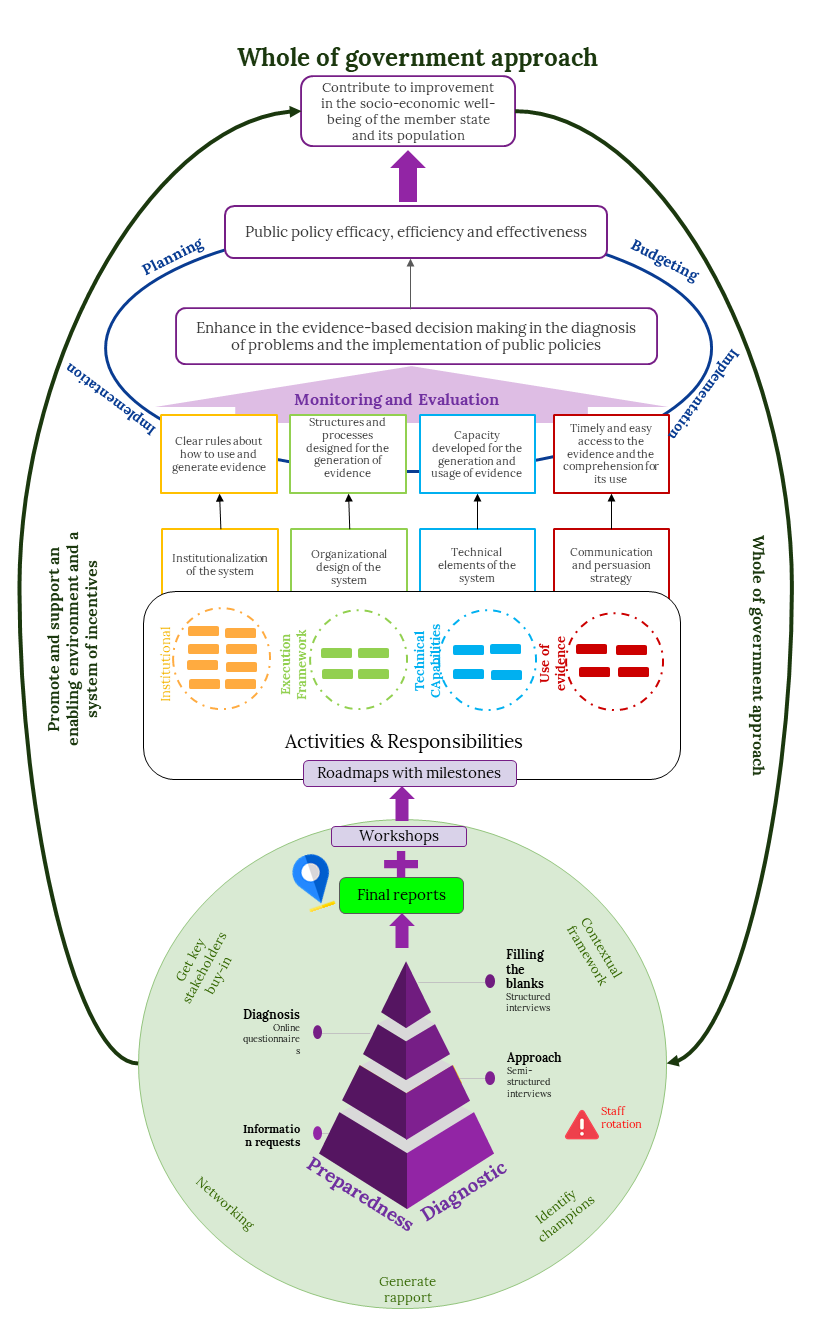
\includegraphics[width=0.75\linewidth]{./images/figure_1} 

}

\caption{Theory of Change}\label{fig:figure1}
\end{figure}

\begin{center}\rule{0.5\linewidth}{0.5pt}\end{center}

As these four dimensions advance and become solid practices, beyond compliance, the system moves towards an increase in evidence-based decision making across government/the institution and across planning, budgeting, and implementation that makes it possible to increase public policies' efficiency, efficacy, and effectiveness.

As the system stays in place and becomes mature, all the dimensions will be strengthened, the enabling environment will advance towards an RBM culture, and all of these will end up contributing to improve the socio-economic well-being of the member state and its population.

\hypertarget{ideal-rbm-system-and-working-process}{%
\section{Ideal RBM system and working process}\label{ideal-rbm-system-and-working-process}}

The development of an RBM System is a complex and nonlinear process that must be contextualized to the specific Member State. To establish a roadmap to strengthen or build an RBM system, the following three elements were considered:

\begin{enumerate}
\def\labelenumi{\arabic{enumi}.}
\tightlist
\item
  A benchmark against which to assess the level of maturity dubbed as ``Ideal RBM System''
\item
  A methodology to obtain general and specific recommendations and,
\item
  A working process and approach to generate ownership
\end{enumerate}

To establish the Ideal RBM system, multiple efforts done over time allow us to learn from experiences in different settings and identify good practices. These good practices represented useful inputs to determine ideal features of an RBM System. The CLEAR LAC team engaged in this collaboration defined four dimensions of an ideal sustainable RBM system (see \protect\hyperlink{fig:figure2}{Figure 2}):

\begin{center}\rule{0.5\linewidth}{0.5pt}\end{center}

\begin{figure}

{\centering 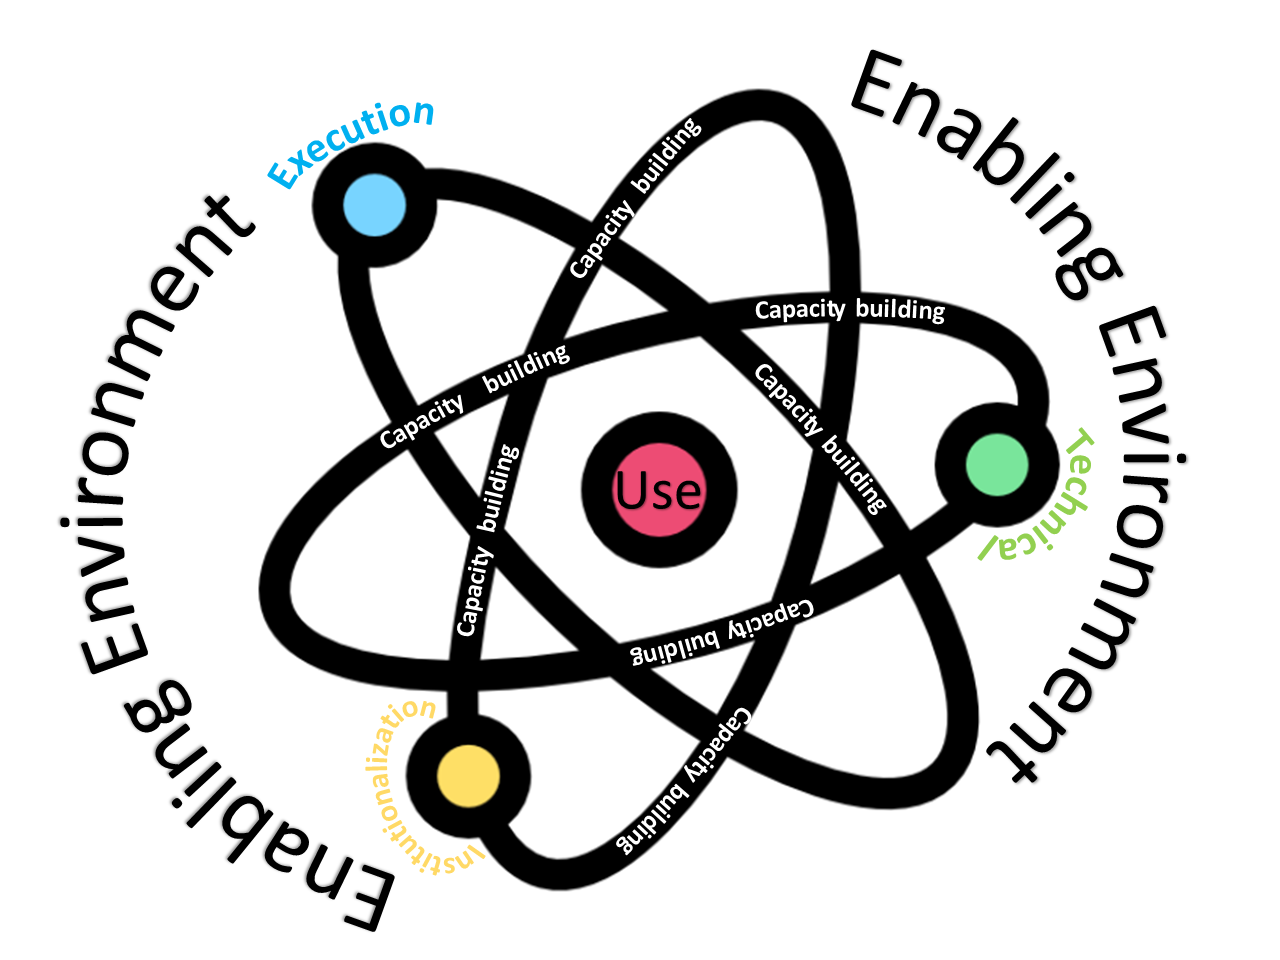
\includegraphics[width=1\linewidth]{./images/figure_2} 

}

\caption{Dimensions of an ideal RBM system}\label{fig:figure2}
\end{figure}

\begin{center}\rule{0.5\linewidth}{0.5pt}\end{center}

\begin{itemize}
\item
  \emph{Institutionalisation:} this dimension focuses on the formal rules that outline the RBM policy in the countries or regional institutions.
\item
  \emph{Execution framework:} this dimension focuses on the systems, resources, processes, methodologies, and tools necessary for the implementation of an RBM system, as well as on the enabling environment.
\item
  \emph{Technical capabilities:} this dimension focuses on the necessary capacities and abilities to implement an RBM System.
\item
  \emph{Use of evidence:} this dimension focuses on the dissemination strategies and incentives aimed at stakeholders with the purpose that they use the evidence generated by the RBM System.
\end{itemize}

Each dimension is integrated by key elements that constitute specific documents, normative frameworks, activities, incentives, among others. These different elements facilitate the operationalisation of the dimension as part of an RBM System. In a third level (beneath dimensions and elements), each element has sub-elements that list their ideal characteristics.

Once all the required information is gathered and analysed (based on the dimension-element-subelement structure) the dimensions will be assessed using a 3-level scale for each sub-element (no, yes, need of improvement)\footnote{For more details on the 3-level scale see \protect\hyperlink{appendixA}{appendix A}} .

For this last step, the progress rate in each sub-element within the element is added end and a cumulative value will be generated to rate the element. Subsequently, all the element values within each dimension are added to determine the progress rate of each dimension.

Finally, the average from the progress of the four dimensions will place each Member State at a specific level of progress (Early initiatives; Committed development; Growing RBM system; Consolidated practices, or Mature state) in the development and implementation of an RBM System (see \protect\hyperlink{appendixA}{Appendix A} for more details).

The working process, defined for this collaboration, identifies Monitoring and Evaluation (M\&E) activities as central elements to be developed and applied in order to affect planning, budgeting, and implementation. \protect\hyperlink{fig:figure3}{Figure 3} presents the working process and highlights the importance of evidence-based decision making (guided and made feasible by M\&E activities and supported, strengthened, and made sustainable through learning and accountability).

\begin{center}\rule{0.5\linewidth}{0.5pt}\end{center}

\begin{figure}

{\centering 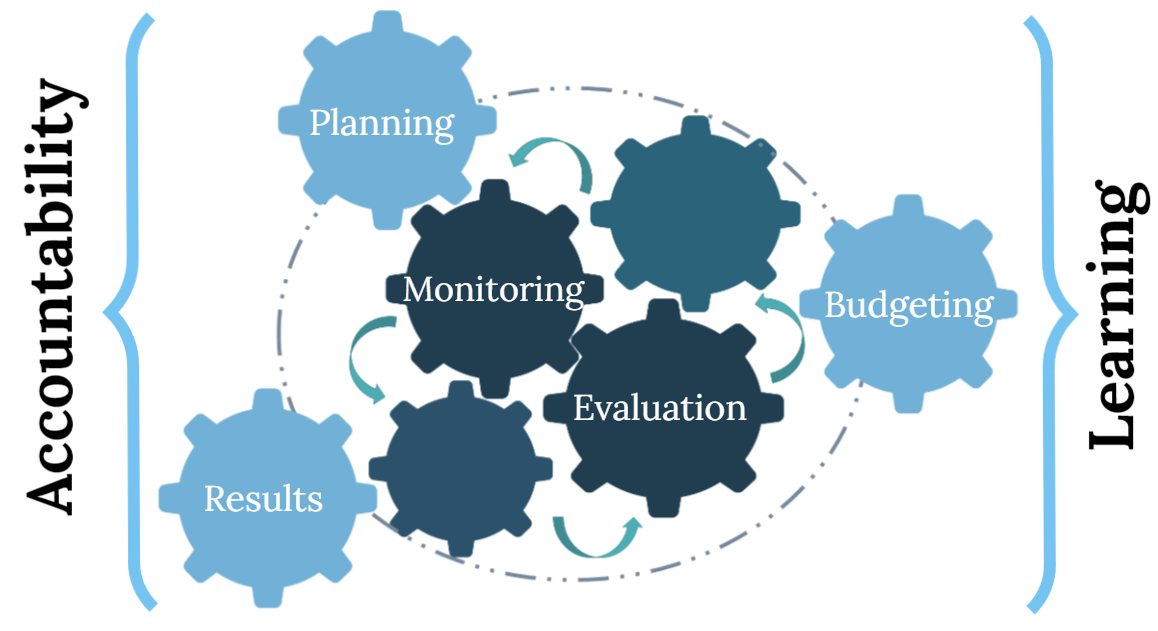
\includegraphics[width=1\linewidth]{./images/figure_3} 

}

\caption{Working Process defined for the CARICOM Collaboration}\label{fig:figure3}
\end{figure}

\begin{center}\rule{0.5\linewidth}{0.5pt}\end{center}

One significant component to strengthen RBM in the Community is to build, in a participatory process, specific roadmaps to continue the development of RBM Systems for each pilot Member State and Regional Institution.

The Member States and Regional Institutions participating in the pilot have relevant but heterogeneous advances achieving this goal. To identify these advances, guide the analysis of the Preparedness Diagnostic stages, and develop ownership, the roadmap will be defined in workshops with key stakeholders involved in different levels (management, coordination, and operation).

\hypertarget{stages-of-the-preparedness-diagnostic}{%
\section{Stages of the Preparedness Diagnostic}\label{stages-of-the-preparedness-diagnostic}}

The Preparedness Diagnostic (PD) is a four-stage methodology designed to gain a deep understanding of the characteristics of the Member State to inform the development of an RBM System.

One main assumption underpinning the methodological design of the PD, is that building a sustainable RBM System requires the active involvement of multiple stakeholders. The PD uses different data collection methods to identify and engage these stakeholders at different stages as well as to obtain information to understand the current policy environment; stakeholder's interests, their roles, motivations, relationship dynamics; map existing institutional structures, practices, and mechanisms; and define capacity building needs.

To successfully execute the PD, the CLEAR LAC team, in collaboration with the CARICOM Secretariat, selected Executive Coordinators who are representatives for the collaboration from the three Member States (Dominica, Jamaica and Saint Lucia) and the three Regional Institutions (the CARICOM Development Fund, the Caribbean Examinations Council and the CARICOM Implementation Agency for Crime and Security).

The role of the Executive Coordinators was key to execute the PD as they have an overall knowledge of their Member State or Regional Institution and have experience in RBM. As Executive Coordinators and key informants, they acted as focal points and contributed to identifying and engaging relevant stakeholders at the different stages of the PD.

\hypertarget{stages-of-the-pd}{%
\subsection*{Stages of the PD}\label{stages-of-the-pd}}
\addcontentsline{toc}{subsection}{Stages of the PD}

The four stages of the PD (presented in \protect\hyperlink{fig:figure4}{Figure 4} ) are implemented according to a specific sequence and were customized based on the findings of the previous stage. They also involve the participation of different stakeholders to obtain a broad perspective of the pilot Member States and Regional Institutions. The figure below provides a brief description of the approach for implementing the stages.

\begin{center}\rule{0.5\linewidth}{0.5pt}\end{center}

\begin{figure}

{\centering 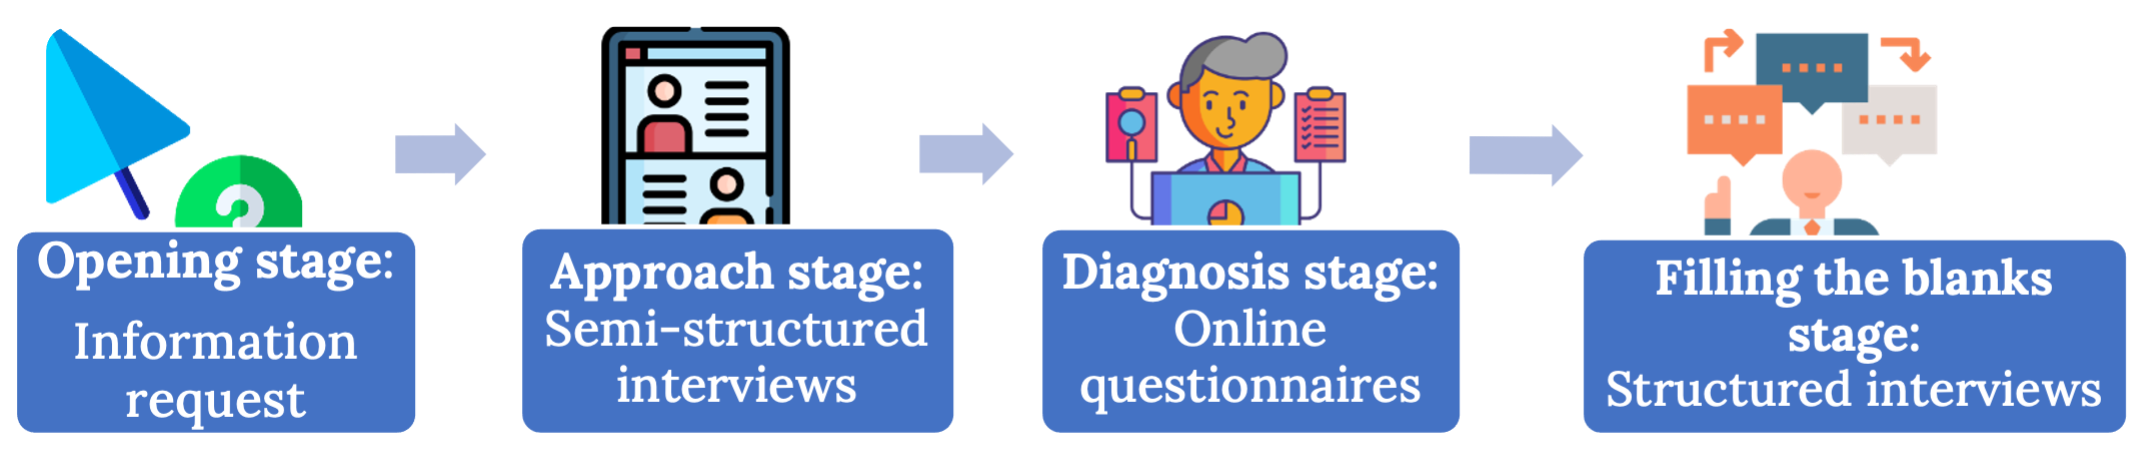
\includegraphics[width=1\linewidth]{./images/figure_4} 

}

\caption{Stages of the Preparedness Diagnostic}\label{fig:figure4}
\end{figure}

\begin{center}\rule{0.5\linewidth}{0.5pt}\end{center}

The \textbf{Opening stage} consisted of a request for different documents from the Executive Coordinators, regarding the pilots' planning, budgeting, and M\&E practices. The desk review and analysis of these documents, in addition to other publicly available information, allowed the design of targeted customized questions for each pilot in the next stage.

The \textbf{Approach stage} involved the identification of various key stakeholders with the support of the Executive Coordinators and the CARICOM Secretariat. The semi-structured interviews addressed general themes that allowed the team to develop rapport with relevant actors within the pilots, as well as obtain additional information about the pilots' current policy environment.

The \textbf{Diagnosis stage} consisted of a series of online questionnaires for the Ministries, Agencies, and Departments of Member States, and Units of Regional Institutions. This stage aimed to gather more in-depth information which would complement information gathered in previous stages and to strengthen the whole of government approach for RBM. The participants were able to respond to questions and upload documents in a timeframe of approximately four weeks, as well as consult with other stakeholders for any additional information within their pilot Member States or Regional Institutions.

Finally, the \textbf{Filling-the-blanks} was aimed at addressing information gaps from the previous stages through a series of structured interviews. This stage targeted other stakeholders such as members of Parliament, representatives of multilateral international organizations, development partners, etc.

\begin{longtable}[]{@{}
  >{\raggedright\arraybackslash}p{(\columnwidth - 4\tabcolsep) * \real{0.1957}}
  >{\centering\arraybackslash}p{(\columnwidth - 4\tabcolsep) * \real{0.3261}}
  >{\raggedleft\arraybackslash}p{(\columnwidth - 4\tabcolsep) * \real{0.4783}}@{}}
\caption{\label{tab:table1} Jamaica's Preparedness Diagnostic Numbers}\tabularnewline
\toprule
\endhead
& \textbf{Stage 1 -- Opening} & Information request to Executive Coordinator + document analysis (+20 documents) + research on official websites. \\
& \textbf{Stage 2 -- Approach} & 4 semi-structured interviews were conducted by the CLEAR LAC team with relevant stakeholders from the Attorney General´s Chambers, Department of Economic Development and Youth Economy and the Ministry of Finance, among others. \\
& \textbf{Stage 3 -- Diagnosis} & +100 online questionnaires were sent to MDAs and were answered with both the whole-of-government and MDA approaches. \\

\includegraphics{./images/tb1_4.png} & \textbf{Stage 4 -- Filling the blanks} & 5 structured interviews were conducted by the CLEAR LAC team with relevant stakeholders from the Ministry of Finance, the Office of the Cabinet, representatives from IFIs, among others. \\
\bottomrule
\end{longtable}

All the information gathered in the four stages was systematized and analysed to present the findings in this document.

\hypertarget{strengths-of-the-pd}{%
\subsection*{Strengths of the PD}\label{strengths-of-the-pd}}
\addcontentsline{toc}{subsection}{Strengths of the PD}

\begin{itemize}
\item
  Different stages designed to identify specific stakeholders and to generate rapport with them.
\item
  As the stages are implemented and analysed sequentially, different layers of information are gathered
\item
  Participatory process that leads to the Member States or RI's ownership of the collaboration
\item
  Qualitative and quantitative mixed methods used
\item
  All stages are adapted for to consider the context of each Member State or RI
\end{itemize}

\hypertarget{limitations-of-the-pd}{%
\subsection*{Limitations of the PD}\label{limitations-of-the-pd}}
\addcontentsline{toc}{subsection}{Limitations of the PD}

\begin{itemize}
\item
  Specific results for one pilot cannot be generalized to others given the customization of the instruments and contextual differences among them
\item
  There are time limitations due to tight agendas of stakeholders that complicates reaching all the desired informants.
\item
  All stages were implemented remotely, and it is preferred to have some face-to-face contact with the stakeholders in at least one of the stages to generate rapport
\item
  The duration of the PD is approximately six effective months; however this was extended due to the whole of government/institution approach and the stakeholders' agendas.
\end{itemize}

\hypertarget{section4}{%
\chapter{Saint Lucia's profile}\label{section4}}

Saint Lucia is an island country in the Caribbean, part of the windward island chain of the eastern Caribbean region, located in the West Indies. It has a population of 186,629 people and a GDP of 1.617 billion as of 2020\footnote{World Bank Data. (2020). St.~Lucia. \url{https://data.worldbank.org/country/st-lucia}}.St. Lucia first achieved a representative government in 1924 and an autonomous internal government as a member of the West Indian Federation until it achieved its independence in 1979, becoming a parliamentary democracy within the Commonwealth\footnote{Tolson, R., Niddrie, D. L., \& Momsen, J. D. (s. f.). Saint Lucia - History. Encyclopedia Britannica. \url{https://www.britannica.com/place/Saint-Lucia/History}}.

As a parliamentary democracy, the head of State is the British monarch, Queen Elizabeth II, who is represented in the country by the governor-general, appointed by the Queen. The head of the government lies with the Prime Minister, who is the leader of the majority party or majority coalition that wins the legislative elections; The legislative branch is made up of the House of Assembly, which has 17 members elected by universal suffrage for a period of five years, and the Senate, which has 11 members appointed by the governor-general. The two major political parties are the Saint Lucia Labour Party and the United Workers Party (UWP).

Last general elections were held in July 2021 and resulted in a massive victory for the SLP, winning 13 over the 17 seats, while the UWP, who had been the party in power since 2016.

These are the fourth consecutive elections in which the incumbent government loses to the opposition, however the country has long experienced peaceful transfers of power between the opposite parties\footnote{Freedom House. (2021). St.~Lucia Overview. \url{https://freedomhouse.org/country/st-lucia/freedom-world/2021}}.

Some of the persistent challenges the country has faced in later years, include government corruption and inadequate transparency as well as a perception of impunity for abuses such as policy brutality and discrimination against minorities\footnote{Freedom House. (2021). St.~Lucia Overview. \url{https://freedomhouse.org/country/st-lucia/freedom-world/2021}}.

Regarding the country's foreign policy, St.~Lucia is part of CARICOM and maintains close relations with the Caribbean countries, and countries with the greatest presence in the region, such as Venezuela, Cuba, Brazil, the United States, the United Kingdom, Canada, France, and Spain. It is also important to mention that St.~Lucia traditionally has been one of the most active countries in advocating for the added value of Caribbean integration\footnote{ Ministerio de Asuntos Exteriores de España. Ficha País Santa Lucía. \url{http://www.exteriores.gob.es/Documents/FichasPais/SANTALUCIA_FICHA\%20PAIS.pdf}}.

\begin{longtable}[]{@{}
  >{\raggedright\arraybackslash}p{(\columnwidth - 4\tabcolsep) * \real{0.1935}}
  >{\centering\arraybackslash}p{(\columnwidth - 4\tabcolsep) * \real{0.4194}}
  >{\raggedleft\arraybackslash}p{(\columnwidth - 4\tabcolsep) * \real{0.3871}}@{}}
\caption[\label{tab:table2} General Statistics of Saint Lucia]{\label{tab:table2} General Statistics of Saint Lucia\footnote{All data was consulted on the World Bank data website: \url{https://data.worldbank.org/indicator}}}\tabularnewline
\toprule
\endhead
& \textbf{Gross Domestic Product} & 1,703M USD (nominal, 2020) Position 188/216 \\
& \textbf{Main economic activities} & Services (86.9\%) Industries (10.9\%) Agriculture (2.2\%) \\
& \textbf{Inflation rate} & 3.8\% (Consumer Price Index) \\
& \textbf{Population} & 184,751 (2021) \\
& \textbf{Poverty} & 20.3\% (headcount ratio at national poverty lines, 2016) \\
\bottomrule
\end{longtable}

\hypertarget{saint-lucia-rbm-profile}{%
\section{Saint Lucia RBM Profile}\label{saint-lucia-rbm-profile}}

The government of Saint Lucia has made efforts to have a system in place where all its MDAs can generate and communicate reports on the most important aspects of planning and budgeting to decision-makers and thus improve the performance of the government. In this way, various frameworks have been created for strategic planning, budgeting, monitoring and evaluation. However, there are still challenges in being able to coordinate monitoring, evaluation, and reporting efforts with those of planning and budgeting.
The planning process, both at the national level and at the MDA level, is clear and the relevant stakeholders and timeframes are identified\footnote{ Saint Lucia´s planning is done in a mid-term basis (there is a Medium-term Development Strategy each triennium)}. Meanwhile, the budgeting process is inertial, that is, resources are systematically distributed to the same priorities and only based on their availability.

The activities and findings of a monitoring and evaluation system and RBM practices have not been able to contribute to improving budgeting and planning decision-making. However, there are efforts that have materialized into good practices within the government, such as the creation of the Project Monitoring Committee for each government project, which seeks to monitor the results of the programs based on the indicators that were raised from the moment of their design; the monitoring and evaluation reports requested from each project within the framework of the Medium-term Development Strategy; the preparation of budget reports based on the templates delivered by the Ministry of Finance where budget ceilings are established, the objectives of each MDA and the programs that seek to achieve those objectives and how it is aligned with national planning.

Despite the efforts by the government of Saint Lucia mentioned above regarding planning, budgeting, and performance management, there seem to be significant deficiencies in articulating them in order to better implement, evaluate, and improve policies, programmes, and projects. Regarding implementation, the government of Saint Lucia, as well as CARICOM Secretariat, are associated with a deficit in terms of policies, programs, projects, and processes (planning, budgeting, adjustments, etc.). This deficit can be seen through the progress rates of the implementation of programs, which are usually around 60\% (or even lower), and whose terms of reference, plans and timeframes are often postponed, generating losses of resources and a lack of confidence of investors and donors in government. In addition, the deficit translates into a sharp decrease in the government's capacity to meet the demands of citizens, as well as the public problems that most afflict the country. In turn, the government's accountability and effectiveness undermine its position vis-a-vis the private, external sectors, and international aid.

As mentioned before, having a whole-of-government RBM system in place and running will have effects on different processes, being planning and budgeting two of the most relevant ones. The government of Saint Lucia has clearly defined planning and budgeting processes (see Appendix C) that should be considered as the national RBM policy is developed; this will help identify specific needs and guide the RBM policy towards its use, privileging timeliness of the information generated. The overall national planning and budgeting processes are briefly explained below:

\hypertarget{national-planning-process}{%
\subsection{National planning process}\label{national-planning-process}}

Saint Lucia´s planning process is consistent over time and identifies the times, resources and personnel necessary to carry it out. Saint Lucia´s planning is done in mid-term basis, and there is no long-term national development plan. However, government´s priorities will be given to the preparation of a Medium-Term Development Strategy (MTDS) which will be the key element in terms of national planning (MTDS includes 6 main sectors: health, tourism, agriculture, infrastructure, citizen security, and education.

There is a proposed investment to achieve these mid-term goals, the majority is oriented to health (46.6\%) and infrastructure (39.5\%). The Ministry of Economic Development, Housing, Urban Renewal, Transport, and Civil Aviation is responsible for national planning. As such, this Ministry plays a pivotal role in the coordination of development planning; mobilisation of public resources; and ensuring effective accountability for the use of such resources for the benefit of all stakeholders.

A participatory approach should be employed in preparing the MTDS and NDP to ensure that the views and ideas of all stakeholders (public, private, NGOs, CBOs, civil society, academia, statutory organisations, etc.) are incorporated. This is essential to ensure ownership of the plan and successful implementation of the various strategies and actions. The MTDS and NDP should also inform the various strategies outlined in the strategic/sector plans of the various line agencies. Additionally, the various sector plans would serve as a guide for Agencies to develop and prioritise projects and programs, which would ultimately feed into the Government's public sector investment programs and successive annual budget estimates\footnote{Planning of Saint Lucia. \url{https://observatorioplanificacion.cepal.org/en/planning-systems/planning-saint-lucia}}.

\hypertarget{national-budgeting-process}{%
\subsection[National budgeting process]{\texorpdfstring{National budgeting process\footnote{The Citizen's Guide to the 2021-2022 budget. Ministry of Finance, Economic Growth, Job Creation, External Affairs and the Public Service. Consulted in: \url{https://www.govt.lc/media.govt.lc/www/pressroom/news/attachments/the-citizen-s-guide-to-the-2021-2022-budget.pdf}}}{National budgeting process}}\label{national-budgeting-process}}

Saint Lucia's budgeting process consists of three main stages: 1. Budget planning and preparation; 2. Finalisation and 3. Budget implementation and monitoring. The stages are comprised as follow.

\hypertarget{budget-planning-and-preparation}{%
\subsubsection{Budget planning and preparation}\label{budget-planning-and-preparation}}

\begin{enumerate}
\def\labelenumi{\arabic{enumi}.}
\item
  The Ministry of Finance (MOF) prepares the Macroeconomic Outlook for the upcoming fiscal year where macroeconomic indicators are reviewed and projections for recurrent revenue, recurrent expenditure, and capital expenditure are formulated.
\item
  A request/call for new initiatives for recurrent revenue, recurrent expenditure as well as capital expenditure are sent to ministries.
\item
  The fiscal targets including economic indicators are established to determine revenue and expenditure projections, which aid in establishing overall spending limits for the new fiscal year.
\item
  The MOF issues the Estimates Call. In this circular, the preliminary allocations are outlined as well as other requirements of the MOF.
\item
  The Minister for Finance invites the private sector to submit inputs for the budget.
\item
  The agencies submit their new initiatives. The MOF reviews the submission and prepares recommendations in consultation with agencies.
\item
  Technical Budget Committee meetings are held with staff of the MOF and Department of Economic Development and Youth Economy to discuss recommendations, indicators and fiscal targets from the Budget Office, Debt Unit, Research Department and Department of Economic Development and Youth Economy. This committee then formulates recommendations and submits to the Budget Policy committee for approval through several iterations.
\end{enumerate}

\hypertarget{finalisation}{%
\subsubsection{Finalisation}\label{finalisation}}

\begin{enumerate}
\def\labelenumi{\arabic{enumi}.}
\setcounter{enumi}{7}
\item
  After extensive reviews and dialogue the MOF present the draft estimates to the Minister for Finance.
\item
  The Minister and Finance Officials meet with Cabinet to finalise the estimates.
\item
  A second call circular is sent to the agencies communicating cabinet final approval of the Budget and changes required to be reflected in the estimates book, and any other relevant instructions.
\item
  Following the Cabinet meeting, MOF prepares the printed estimates and develops the budget papers.
\item
  The Ministry for Finance prepares and submits a draft appropriation bill to the Attorney General
\item
  The Attorney General reviews the Appropriation Bill and prepares the Resolution.
\item
  Minister for Finance tables the Resolution in the House of Parliament.
\item
  Members of the Lower House debate the Estimates.
\item
  The Appropriation Bill is tabled and debated.
\item
  When passed the Appropriation Act is then assented to by the Governor-General and Gazetted.
\end{enumerate}

\hypertarget{budget-implementation-and-monitoring}{%
\subsubsection{Budget implementation and monitoring}\label{budget-implementation-and-monitoring}}

\begin{enumerate}
\def\labelenumi{\arabic{enumi}.}
\setcounter{enumi}{17}
\item
  The MOF sends out a call to agencies to submit their expenditure request (recurrent expenditure, capital), revenue (actual and projections), and procurement plans on a quarterly basis.
\item
  The MOF releases the allocation to agencies on a quarterly basis. The release of allocation is based in part on the current revenue performance and projections for the year. Capital expenditure allocation is determined based on the availability of the loan, grant, bond, or other fundraising and the status of the projects.
\item
  Agencies are required to submit monthly revenue reports and quarterly performance reports to the MOF.
\item
  The MOF is also required to produce and submit quarterly performance reports to the Minister for Finance.
\end{enumerate}

\hypertarget{section5}{%
\chapter{Main findings}\label{section5}}

As mentioned above, this Preparedness Diagnostic uses as a reference a four dimensions/bundles analysis, each one contains elements considered relevant to have an ``Ideal RBM System''. This Ideal RBM System serves as a benchmark that allow to compare the current situation in Saint Lucia in relation to the best possible scenario regarding practices, uses, and results of RBM. In this way, figure 5 shows the rate of progress that Saint Lucia has in each of the dimensions of analysis, with respect to the ideal scenario.

The elements and sub-elements of the reference Ideal RBM System are not usually part of the status quo, they should be identified, designed and developed; following this, a country that has not considered adopting RBM practices would probably not comply or show advances in any of the analysed elements. In this sense, all the advances identified in this diagnosis represent valuable progress.

It is important to mention that, although there is a numerical value for each dimension, behind the numbers there was a qualitative analysis that determined the current situation of Saint Lucia regarding RBM. Furthermore, these ``ratings'' are in terms of the ideal scenario, so in no way does it represent an outright success or failure, but rather an approximation to the best possible situation of the RBM.

\begin{longtable}[]{@{}
  >{\raggedright\arraybackslash}p{(\columnwidth - 2\tabcolsep) * \real{0.3889}}
  >{\raggedright\arraybackslash}p{(\columnwidth - 2\tabcolsep) * \real{0.3472}}@{}}
\toprule
\begin{minipage}[b]{\linewidth}\raggedright
DIMENSION
\end{minipage} & \begin{minipage}[b]{\linewidth}\raggedright
LEVEL OF PROGRESS
\end{minipage} \\
\midrule
\endhead
INSTITUTIONALISATION & 9\% \\
EXECUTION FRAMEWORK & 3\% \\
TECHNICAL CAPABILITIES & 3\% \\
USE OF EVIDENCE & 14\% \\
\bottomrule
\end{longtable}

\begin{figure}

{\centering 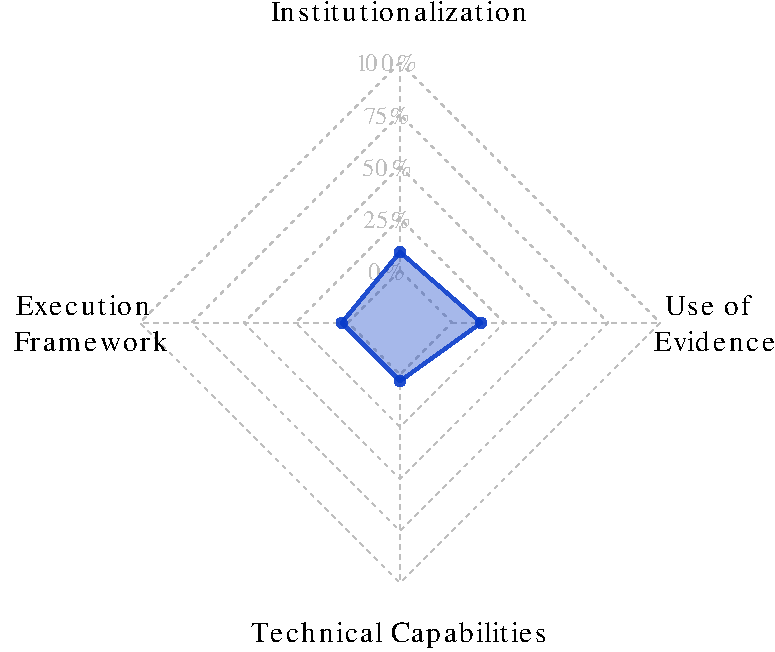
\includegraphics[width=0.7\linewidth]{_main_files/figure-latex/figure5-1} 

}

\caption{Level of progress of the Ideal RBM System}\label{fig:figure5}
\end{figure}

Considering this rate of progress, a metric was built to progressively identify five levels of maturity of RBM systems. In this way, the data presented above are averaged and a graph is generated for all the dimensions and a graph that contains the average of the dimensions, identifying the level in which the country falls . The 5 levels are:

\begin{enumerate}
\def\labelenumi{\arabic{enumi}.}
\tightlist
\item
  Early initiatives
\item
  Committed development
\item
  RBM System
\item
  Consolidated practices
\item
  Mature State
\end{enumerate}

For the case of Saint Lucia, the findings regarding the level of maturity of its RBM system are the following:

Saint Lucia is currently at the Early initiatives level. This occurs because even though the country has a few RBM tools and activities in place within the government, they are not articulated and regulated by any guideline, so they are also not incorporated in the planning and budgeting processes.

However, as mentioned before, this does not mean that Saint Lucia's efforts will be dismissed in some way, but rather that we will be able to find the starting point to build a strong RBM system that considers the country's contextual factors so that Saint Lucia gets closer and closer to the ideal scenario.

\hypertarget{results-by-dimension}{%
\section{Results by dimension}\label{results-by-dimension}}

The results of this diagnosis for each of the dimensions analysed (and their ideal elements) are presented below in a synthetic manner. For more detailed information on each dimension, elements, and sub-elements, please see \protect\hyperlink{appendixB}{appendix B} and visit the interactive platform with all the disaggregated findings of this PD.

\hypertarget{institutionalisation}{%
\subsection{Institutionalisation}\label{institutionalisation}}

\textbf{Key Message:}
Saint Lucia has institutionalized planning and budgeting processes. Its medium-term planning has key results areas and these, in turn, have clear monitoring indicators, although they focus on outputs, not outcomes. However, the necessary mechanisms do not exist to formally establish who (relevant coordination and operation actors), how (methodologies) and when (timeframes) will carry out the M\&E and RBM activities to improve decision-making and thus obtain the desired results. Therefore, there is not an integrated normative framework for RBM and M\&E in the country.

\begingroup\fontsize{12}{14}\selectfont

\begin{tabu} to \linewidth {>{\raggedright}X>{\raggedright}X}
\hline
Ideal Element & Main results/findings\\
\hline
\textbf{1. There is a documented, approved and binding RBM Policy within the government} & In Saint Lucia there is no RBM legislation nor policies that delegate RBM to a government body. The Department of Economic Development and Youth Economy and the Department of Finance lead RBM activities in the country, but not according to formal laws and procedures.\\
\hline
\textbf{2. There are laws/regulations/norms recognizing M\&E activities across the government} & There are no laws/regulations/norms recognizing M\&E activities across the government.\\
\hline
\textbf{3. There are guidelines that establish the rules and processes to perform monitoring activities} & Although there are no guidelines that establish the rules and processes to perform monitoring activities across government, there are monitoring activities regarding the development strategies of the government.\\
\hline
\textbf{4. There are guidelines that establish the rules and processes to perform evaluation activities} & There are no guidelines that establish the rules and processes to perform evaluation activities.\\
\hline
\textbf{5. There are guidelines that establish the rules and processes to address and use M\&E results} & There are no guidelines that establish the rules and processes to address and use of M\&E results.\\
\hline
\textbf{6. There are formal actions towards building an enabling environment} & Although there is an interest coming from the government of Saint Lucia to have an RBM system in place, there have been no formal efforts to institutionalize the development and use of M\&E and RBM tools and activities.\\
\hline
\textbf{7. There is a Results Oriented National Plan defined for a given period in the country} & Although there is no long-term National Development Plan, Saint Lucia has worked with mid-term development strategies. The current mid-term development strategy is the Medium-Term Development Strategy 2020 - 2023 and it identifies six Key Results Areas: Agriculture, Citizen Security, Education, Healthcare, Infrastructure and Tourism. Now the drafting of the period up to 2026 is in progress.\\
\hline
\textbf{8. There is a national budgeting strategy for a given period in the country} & The national budgeting process of Saint Lucia consists of three main sub-processes: Budget Planning and Preparation, Budget finalisation and the Budget Implementation and Monitoring. And there is also a Citizen's Guide to the budget.\\
\hline
\end{tabu}
\endgroup{}

\hypertarget{execution-framework}{%
\subsection{Execution Framework}\label{execution-framework}}

\textbf{Key Message:}
Saint Lucia has personnel dedicated to monitoring projects within the MDAs, such as the Project Monitoring Committee and the chief economists. However, these groups do not usually carry out monitoring and evaluation activities in a systematic way and are not coordinated or articulated with the planning, budgeting, and implementation processes to improve the results of the MDAs. In addition, in the MDAs there are no defined processes or specific resources allocated, nor a common language on M\&E and RBM.

\begingroup\fontsize{12}{14}\selectfont

\begin{tabu} to \linewidth {>{\raggedright}X>{\raggedright}X}
\hline
Ideal Element & Main results/findings\\
\hline
\textbf{9. There are operative handbooks to implement the monitoring functions (i.e., Logic Framework)} & There are no operative guidelines/handbooks/norms regarding Monitoring functions. However, there are some informal monitoring functions within MDAs.\\
\hline
\textbf{10. There are operative handbooks that establish specific steps to develop each stage of the evaluation function} & As there are no operative guidelines/handbooks/norms/informal activities regarding Evaluation functions, stages of the evaluation process are not identified.\\
\hline
\textbf{11. There is an operating and functioning coordination of M\&E at the national or/and subnational levels} & There is no M\&E system at the national or/and subnational levels in Saint Lucia.\\
\hline
\textbf{12. There is a defined human resources structure for M\&E activities} & Despite there are Project Monitoring Committees, in charge of gathering information regarding projects undertaken by MDAs, there is no defined human resources structure for M\&E activities within Saint Lucia´s government.\\
\hline
\end{tabu}
\endgroup{}

\hypertarget{technical-capabilities}{%
\subsection{Technical capabilities}\label{technical-capabilities}}

\textbf{Key Message:}
There is no sufficient offer (both private or public) or demand (from the government) for M\&E services and capacity building in RBM within Saint Lucia. Also, there are no sufficient skilled personnel within the government with the capability to identify M\&E needs and conduct M\&E activities with the objective of orienting planning and budgeting towards results.

\begingroup\fontsize{12}{14}\selectfont

\begin{tabu} to \linewidth {>{\raggedright}X>{\raggedright}X}
\hline
Ideal Element & Main results/findings\\
\hline
\textbf{13. There are sufficient private and public entities providing M\&E services, including training, to the public sector} & There are insufficient private and public entities providing M\&E services, including training to the public sector.\\
\hline
\textbf{14. There are skilled personnel in government with technical capacity and competencies to conduct planning and budgeting for results} & There are nosufficient skilled personnel in government with technical capability and competencies to conduct planning and budgeting for results.\\
\hline
\textbf{15. There are skilled personnel in government with technical capacity and competencies to conduct monitoring activities} & Although there are personnel doing some monitoring activities (of programmes and projects mainly), there are no sufficient skilled personnel in government with technical capability and competencies to conduct monitoring activities.\\
\hline
\textbf{16. There are skilled personnel in government with technical capacity and competencies to conduct evaluations and evaluation activities} & There are no sufficient skilled personnel in government with technical capacity and competencies to conduct evaluations and evaluation activities.\\
\hline
\end{tabu}
\endgroup{}

\hypertarget{use-of-evidence}{%
\subsection{Use of evidence}\label{use-of-evidence}}

\textbf{Key Message:}
Saint Lucia has planning and budgeting information publicly available, but not regarding government performance. Although there are efforts to monitor and use its results, such as the Project Monitoring Committee, there are just compliance-oriented and not results-oriented. As there are no evaluation activities, there is no use regarding evaluation findings/evidence. Also, a strategy to generate a culture of evidence use is not identified.

\begingroup\fontsize{12}{14}\selectfont

\begin{tabu} to \linewidth {>{\raggedright}X>{\raggedright}X}
\hline
Ideal Element & Main results/findings\\
\hline
\textbf{17. RBM documents and government performance information are available and accessible for consultation} & National planning and budgeting documents are publicly available, such as the Medium-Term Development Strategies, and the Citizen's Guide to the 2021-2022 Budget where indicators can be found and then tracked in order to measure performance. However, there are no documents publicly available with information on government performance.\\
\hline
\textbf{18. There is an enabling environment for the use of M\&E results} & There are heterogeneous incentives for the use of monitoring results. Although there are efforts to generate and use the information derived from the monitoring of government projects, as in the case of the Project Monitoring Committee, there are no incentives for them to be recognized by decision-makers. Monitoring results are not necessarily binding within the government. In addition to this, by not having personnel dedicated to monitoring programs, projects and activities, the incentives for its use are very few, being almost nil.\\
\hline
\textbf{19. M\&E results are systematically included in the planning and budgeting} & As there are no mechanisms (both formal or informal) to do so, M\&E results are not systematically included in the planning of Saint Lucia´s programmes, policies, and projects. Regarding budgeting, although some MDAs use the budget templates that ask for budget allocation accordingly to objectives, there is not a mechanism to include M\&E information in the budgeting process.\\
\hline
\textbf{20. The government has mechanisms to measure the use of the evidence that the RBM system generates} & Saint Lucia´s government does not have mechanisms in place to measure the use of the evidence that the RBM (or M\&E) system generates.\\
\hline
\end{tabu}
\endgroup{}

\hypertarget{main-challenges-to-strengthen-the-rbm-system}{%
\section{Main challenges to strengthen the RBM system}\label{main-challenges-to-strengthen-the-rbm-system}}

As mentioned in \protect\hyperlink{section2}{section 2.2}, the development of an RBM System is a complex, nonlinear, and continuous process that must be contextualized in each country. In doing so, it is important to consider the main challenges that Dominica faces when it comes to strengthening its RBM system. This diagnosis identifies three major challenges:

\begin{enumerate}
\def\labelenumi{\arabic{enumi}.}
\item
  Changing the culture and fostering the enabling environment to have an RBM system in place implies a change of mindset of public servants at all levels. It should be considered that throughout the process there must be a constant awareness/sensitization strategy, both in the short and medium term, that allows public servants to identify the importance to have this mindset change in pursuit of RBM. In other words, on a regular basis, there needs to be reminders on the importance of RBM and its impact on improving performance and lives of all citizens.
\item
  Since this collaboration constitutes a whole-of-government approach, it is necessary to have a top-down commitment in which leaders and decision-makers demonstrate the benefits of the RBM system through evidence informed actions that are generated by the RBM system. This means that a top-down approach should be used demonstrate its usefulness of the information and evidence derived from the RBM system in improving the planning and budgeting decisions. Also, considering the whole-of-government approach, a coordination strategy that speaks to this scope should be prioritized to get the expected results and leave the silo approach behind.
\item
  For the RBM system to be sustainable, it is critical to generate a system of incentives and ensure that there is a balance between positive and negative incentives (such as potential penalties for non-compliance), to advance and sustain the system. The positive incentives can take different forms, from monetary to symbolic actions, such as the presentation of awards to staff and units and recognition for good performance in public service.
\end{enumerate}

During the diagnosis it was mentioned several times that the scarcity of financial resources is a major impediment to the formalization of M\&E and RBM activities. However, to start building an RBM system, it is important to be aware that public servants can receive benefits beyond monetary ones, such as recognition of their work within the public sector, whose ultimate value is improving the quality of life of the citizens.

\hypertarget{section6}{%
\chapter{Next steps to building the roadmap}\label{section6}}

RBM entails more than compliance to specific requirements. Compliance is just not enough; it has to do with a change of mindset on the way things are done. This change of mindset involves different areas and stages of the administration. Having reviewed the main results from the Preparedness Diagnostic in terms of the dimensions of elements considered as part of an ideal RBM system, this section introduces the next steps that will be carried out as part of the process of building contextualized roadmaps.

The roadmap will present pathways to influence planning, budgeting, implementation, and the M\&E functions, as well as accountability and learning promotion. The main objective is for Saint Lucia to have a defined action course that also specifies responsibilities and shows the importance of the participation of all relevant stakeholders.

\begin{center}\rule{0.5\linewidth}{0.5pt}\end{center}

\begin{figure}

{\centering 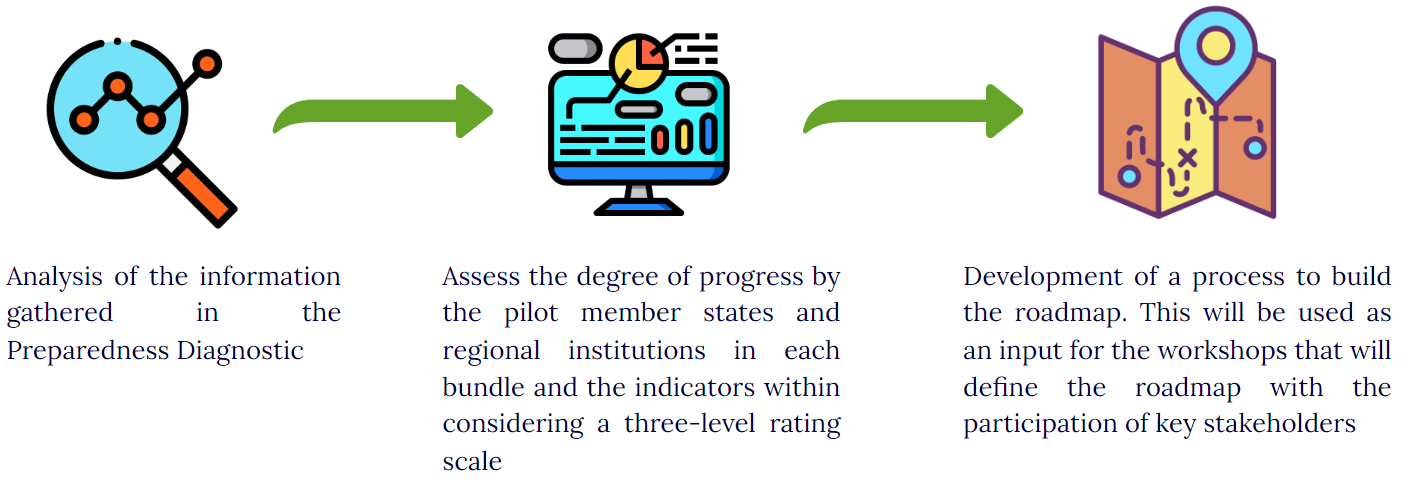
\includegraphics[width=1\linewidth]{./images/figure_6} 

}

\caption{From an ideal RBM system to the roadmaps}\label{fig:figure6}
\end{figure}

\begin{center}\rule{0.5\linewidth}{0.5pt}\end{center}

The whole process has a coproduction approach, were aside of the CARICOM Secretariat, and the Executive Coordinators, key stakeholders will be involved in a fluid process to develop a learning loop that provides feedback and improves the process.

\begin{center}\rule{0.5\linewidth}{0.5pt}\end{center}

\begin{figure}

{\centering 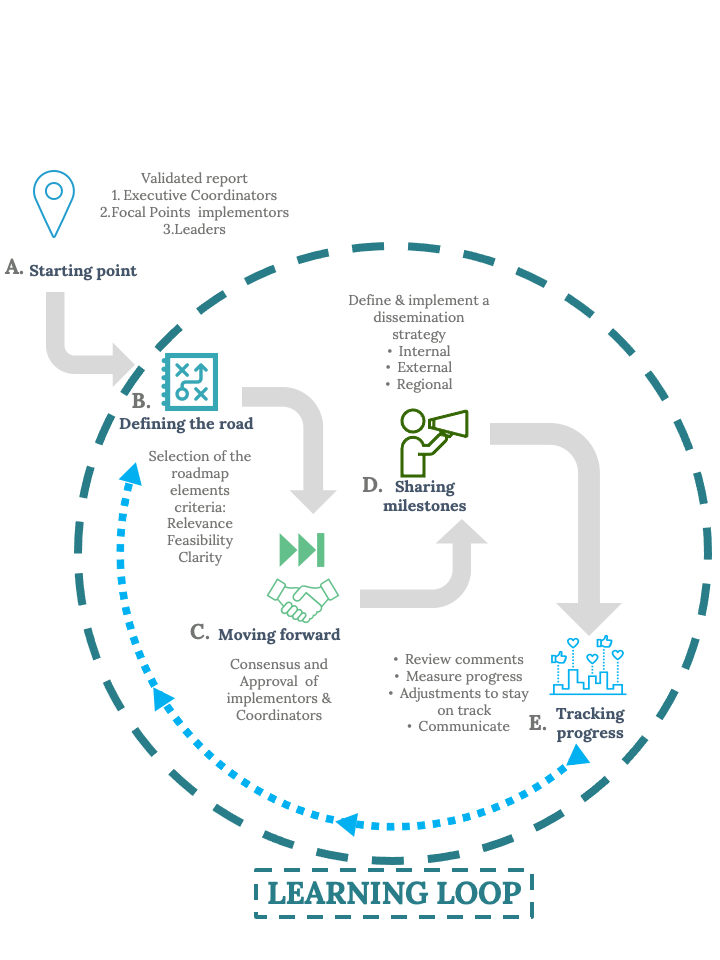
\includegraphics[width=0.75\linewidth]{./images/figure_7} 

}

\caption{Learning loop}\label{fig:figure7}
\end{figure}

\begin{center}\rule{0.5\linewidth}{0.5pt}\end{center}

This report is considered as the \emph{starting point} in this process; take into consideration that, as \protect\hyperlink{fig:figure7}{figure 7} illustrates, the process started before its publication.

Once the first draft was completed, it will be shared with key stakeholders for review and validation, starting with the Executive Coordinators. Once the feedback period concluded, the report itself became an input for what is to come and will be distributed with multiple purposes (including generating knowledge, aiding in empowering key stakeholders in the path of strengthening RBM practices, and promoting appropriation of the next steps).

The next steps start with \emph{defining the road}, engaging key stakeholders to coproduce contextualized mid-term roadmaps that will include specific activities and milestones that sought to materialize their implementation. To develop the roadmap, the CLEAR LAC team has designed a series of workshops with the participation of stakeholders involved in the different areas and levels of what is to be the national RBM system, and that have been carefully identified as part of the Preparedness Diagnostic process.

To \emph{move forward}, this first draft of the roadmap is presented to other relevant stakeholders to build a consensus and support for the process. It is crucial to gain whole-of-government ownership, so it is important to define and implement a dissemination strategy for \emph{sharing clearly define milestones} in different levels: internal, external, and regional once they have been clearly defined and responsibilities have been assigned. Finally, it is important to \emph{track the progress} of implementation and communicate results to assure that the Member State learns from the process, adjusts, and stays on the recommended path, as well as communicating results. The continuum process of identifying, sharing, reviewing, and adjusting represents a learning loop.

\hypertarget{stakeholders-contribution-analysis}{%
\section{Stakeholders' contribution analysis}\label{stakeholders-contribution-analysis}}

This section presents an analysis of stakeholders to identify which of them are relevant to strengthening the RBM system, identifying the main actors that should be involved in the process. Each of these stakeholders are involved in the decision making and execution at varied levels. Based on the CLEAR LAC's team analysis, a proposal of the possible contribution of the stakeholders (considering positions and experience) is summarised below to support the improvement of the system which will generate the necessary evidence and results for decision-making regarding planning, and budgeting and thus achieve the expected results of the Government of Sain Lucia is presented here based on the CLEAR LAC's team analysis considering their positions and experience.

The analysis is summarized (but not limited only, due to the constant change in the dynamics in which the stakeholders relate) in the following table. During the roadmap development workshops that will be held with government stakeholders, new stakeholders could be identified or some of those presented here could be discarded.

\begin{table}

\caption{\label{tab:unnamed-chunk-8}Stakeholders’ contribution analysis}
\centering
\fontsize{12}{14}\selectfont
\begin{tabu} to \linewidth {>{\raggedright}X>{\raggedright}X>{\raggedright}X}
\hline
Stakeholder / Position & Responsibilities / Role in the system & Incentives to be part of the system\\
\hline
\textbf{Cabinet Secretary} & •Under the direction of the Prime Minister, the Cabinet Secretary is responsible for the development, approval, and implementation of the RBM across government & •Good performance of MDAs (oversee, promote and communicate)\\
\hline
\textbf{} & •Provides direction and guidance to the development and implementation of RBM frameworks and guidelines and outputs of the RBM & \\
\hline
\textbf{} & •Provide leadership guidance and direction to Permanent Secretaries on the implementation of RBM & \\
\hline
\textbf{} & •Reviews the performance of Permanent Secretaries in accordance with the government´s performance guidelines & \\
\hline
\textbf{CARICOM Secretariat} & •Demand better results from the Government of Saint Lucia, as well as transparency and accountability & •Achieve better results to the region\\
\hline
\textbf{} & •Develop incentives for the good Member States & •Accountability to donors and governments\\
\hline
\textbf{} & •Create a best RBM practice repository and disseminate them among the Member States & \\
\hline
\textbf{} & • Generate spaces for the exchange of these best practices in the region (knowledge management) & \\
\hline
\textbf{Citizens} & •Demand better results from the government and transparency of its processes & Not Applicable\\
\hline
\textbf{Corporate Planning Units} & •Be the RBM Champions within their MDAs & •Fulfil what is expected from them regarding their responsibilities (planning and reporting on MDA performance)\\
\hline
\textbf{} & •Their primary function is to facilitate the efficient implementation of the Policy and results-based management practices in their respective MDAs & \\
\hline
\textbf{} & •Identify the M\&E needs of their MDAs & \\
\hline
\textbf{} & •Communicate the M\&E needs of their MDA with the RBM system coordinators & \\
\hline
\textbf{} & •Execute M\&E plans within MDAs & \\
\hline
\textbf{Ministries, Departments and Agencies} & • The assessment and building of capacity within their organisations to operate efficiently and effectively in accordance with the RBM Policy requirements & •Comply with all the goals/results proposed in the planning of the MDA\\
\hline
\textbf{} & •Support the Change Management /transition implementation of MDAs to operating RBM Frameworks systems and approaches including: & •Get more resources for their institutions\\
\hline
\textbf{} & •Development of plans in accordance with the Government Integrated Planning Framework and aligned to the National Development Plan (NDP) & •Be recognized for good performance\\
\hline
\textbf{} & •Formulation of budgets in accordance with the MTRBB Framework & •Become the leaders of the sectors in which they operate\\
\hline
\textbf{} & •The building of results, monitoring and evaluation systems/frameworks in their organisations & \\
\hline
\textbf{} & •Performance Management and Accountability Systems/frameworks effectively applied in their organisations & \\
\hline
\textbf{} & •Management Information systems, performance measurement strategies, reporting, capacity, and governance structures in MDAs are consistent with the objectives of the RBM Policy/system & \\
\hline
\textbf{} & •Consider the information derived from M\&E activities in the decision-making processes & \\
\hline
\textbf{} & •Give feedback on the M\&E processes & \\
\hline
\textbf{Ministry of Finance \& Public Service} & •Operationalize the monitoring and evaluation exercise, together with the Ministry of Economic Development and the Performance Management and Delivery Unit (Office of the Prime Minister) & •Become the leader of the results-oriented budgeting across all government\\
\hline
\textbf{} & •Define the universe of monitoring and evaluation (what to monitor and evaluate, periodicity, why) & •Build a strong government by strengthening the way the resources are used\\
\hline
\textbf{} & •Coordinate with the Performance Management and Delivery Unit and the Department of Economic Development and Youth Economy so as not to overlap monitoring objects and monitoring periods & \\
\hline
\textbf{} & •Define mechanisms to comprehensively monitor and evaluate programs & \\
\hline
\textbf{Parliament} & Review and approval of: & •Fulfil the government's counterbalancing function\\
\hline
\textbf{} & • Whole of Government Business Plan aligned to the National Budget & \\
\hline
\textbf{} & • Whole of Government Performance Report & \\
\hline
\textbf{} & • Whole of Government Evaluation Agenda & \\
\hline
\textbf{} & Review of: & \\
\hline
\textbf{} & • Strategic Business Plan of MDAs & \\
\hline
\textbf{} & • MDA Performance Reports & \\
\hline
\textbf{} & • MDA, Project Programme Evaluation Reports & \\
\hline
\textbf{} & • Demand and use M\&E information/findings to incorporate them in the parliamentary decision-making & \\
\hline
\textbf{Performance Management and Delivery Unit (Office of the Prime Minister)} & • Operationalize the monitoring and evaluation exercise, together with the Ministry of Finance and the Ministry of Economic Development & •Become the execution arm of the Prime Minister regarding RBM and M\&E\\
\hline
\textbf{} & •Define the universe of monitoring and evaluation (what to monitor and evaluate, periodicity, purposes) & \\
\hline
\textbf{} & • Coordinate with the Ministry of Finance and the Department of Economic Development and Youth Economy so as not to overlap monitoring objects and monitoring periods & \\
\hline
\textbf{} & • Define mechanisms to comprehensively monitor and evaluate programs & \\
\hline
\textbf{Permanent Secretaries (board)} & •Be responsible for ensuring that RBM and M\&E activities are effectively carried out within their MDAs & • Good performance of their respective MDAs (responsibility of the performance of MDAs)\\
\hline
\textbf{} & •Appoint the RBM champions within MDAs & \\
\hline
\textbf{Prime Minister} & • As the Chief Executive is the Sponsor/Champion for the development and implementation of the RBM Policy & • Whole of Government performance improved\\
\hline
\textbf{} & • Provide policy direction with respect to the development of the results Based Management across the Public Sector & • Improve the perception that citizens have regarding the performance of the government\\
\hline
\textbf{} & • Instruct the actions of the RBM and appoint system coordinators & •Improve confidence/trust with the external sector: investors, donors, etc.\\
\hline
\textbf{} & • Disseminate the RBM strategy to the public & \\
\hline
\textbf{Project Monitoring Committees} & •Identify the M\&E needs of Saint Lucia´s government projects & •Improve decision making within projects\\
\hline
\textbf{} & •Execute M\&E plans & •Identify areas for budget improvements and avoid wasting resources\\
\hline
\textbf{} &  & •Keep projects on time\\
\hline
\textbf{} &  & •Improve projects´ results\\
\hline
\textbf{PS of the Ministry of Economic Development} & •The Department of Economic Development and Youth Economy & •Being the leading planning institution in Saint Lucia, having mechanisms to improve planning decision-making is a tangible incentive\\
\hline
\textbf{} & •Oversee and evaluate project reports to determine compliance with plans & \\
\hline
\textbf{Universities} & •Use the results of the M\&E processes & •Offer RBM/M\&E training to public servants (increase earnings)\\
\hline
\textbf{} & •Participate in the M\&E processes of the government & •Offer RBM/M\&E services to government (increase earnings and strengthening the community of practice in the country and the \vphantom{1} region)\\
\hline
\textbf{} & •Offer M\&E services both in training and monitoring and evaluating \vphantom{1} & \\
\hline
\textbf{} & •Demand evidence derived from M\&E \vphantom{1} & \\
\hline
\textbf{} & •Keep the Government accountable \vphantom{1} & \\
\hline
\textbf{VOPE (Caribbean Evaluators International)} & •Use the results of the M\&E processes & •Offer RBM/M\&E training to public servants (increase earnings)\\
\hline
\textbf{} & •Participate in the M\&E processes of the government & •Offer RBM/M\&E services to government (increase earnings and strengthening the community of practice in the country and the region)\\
\hline
\textbf{} & •Offer M\&E services both in training and monitoring and evaluating & \\
\hline
\textbf{} & •Demand evidence derived from M\&E & \\
\hline
\textbf{} & •Keep the Government accountable & \\
\hline
\multicolumn{3}{l}{\rule{0pt}{1em}\textit{Note: }}\\
\multicolumn{3}{l}{\rule{0pt}{1em}Developed by the CLEAR LAC technical team in charge of the collaboration}\\
\end{tabu}
\end{table}

\hypertarget{references-sources}{%
\chapter*{References \& Sources}\label{references-sources}}
\addcontentsline{toc}{chapter}{References \& Sources}

\begin{itemize}
\item
  World Bank Data. (2020). St.~Lucia. \url{https://data.worldbank.org/country/st-lucia}
  Food and Agriculture Organization of the
\item
  United Nations.https://www.fao.org/investment-learning-platform/themes-and-tasks/results-based-management/en/\#c309481
\item
  Freedom House. (2021). St.~Lucia Overview. \url{https://freedomhouse.org/country/st-lucia/freedom-world/2021}
\item
  Freedom House. (2021). St.~Lucia Overview. \url{https://freedomhouse.org/country/st-lucia/freedom-world/2021}
\item
  Planning of Saint Lucia. \url{https://observatorioplanificacion.cepal.org/en/planning-systems/planning-saint-lucia}
\item
  The Citizen's Guide to the 2021-2022 budget. Ministry of Finance, Economic Growth, Job Creation, External Affairs and the Public Service. Consulted in: \url{https://www.govt.lc/media.govt.lc/www/pressroom/news/attachments/the-citizen-s-guide-to-the-2021-2022-budget.pdf}
\item
  Tolson, R., Niddrie, D. L., \& Momsen, J. D. (s. f.). Saint Lucia - History. Encyclopedia Britannica. \url{https://www.britannica.com/place/Saint-Lucia/History}
\item
  United Nations Development Group. Results-Based Management Handbook. \url{https://unsdg.un.org/download/160/246\#}:\textasciitilde:text=RBM\%20is\%20a\%20management\%20strategy,higher\%20level\%20goals\%20or\%20impact).
\item
  United Nations Development Programme. Results Based Management. Concepts and Methodology. \url{http://web.undp.org/evaluation/documents/RBMConceptsMethodgyjuly2002.pdf}
\end{itemize}

The rest of the sources are official websites of the Government of Saint Lucia or regional institutions/initiatives, such as (but not limited only):

\begin{itemize}
\item
  Government of Saint Lucia. \url{https://www.govt.lc/}
\item
  Cabinet of Ministers. \url{https://www.govt.lc/cabinet-rejected}
\item
  Departments of the Government of Saint Lucia. \url{https://www.govt.lc/departments} (and all the microsites located in this page)
\end{itemize}

\hypertarget{appendix-appendix}{%
\appendix}


\hypertarget{appendixA}{%
\chapter{Conceptual framework (CLEAR LAC)}\label{appendixA}}

\hypertarget{key-dimensions-of-a-sustainable-rbm-system}{%
\section{Key dimensions of a sustainable RBM System}\label{key-dimensions-of-a-sustainable-rbm-system}}

The development of an RBM System is a complex and nonlinear process that must be contextualized to the specific region, country, or regional institution. However, the multiple efforts done over time allow us to learn from experiences in different settings and identify good practices. These good practices represent useful inputs to be considered when embarked on this road.

One significant component to strengthen RBM in the Community is to build, in a participatory process, specific roadmaps to continue the development of RBM Systems for each pilot member state and regional institution. The member states and regional institutions participating in the pilot have significant but heterogeneous advances achieving this goal. To identify these advances and guide the analysis of the Preparedness Diagnostic stages, the CLEAR LAC team defined four dimensions of an ideal and sustainable RBM System:

\begin{itemize}
\item
  \emph{Institutionalisation:} this dimension focuses on the formal rules that defines, outlines and formalize the RBM Systems in the countries.
\item
  \emph{Execution framework:} this dimension focuses on the systems, resources, processes, methodologies, and tools necessary for the implementation of the RBM system, as well as incentives that promote an enabling environment.
\item
  \emph{Technical capabilities:} this dimension focuses on the capacities, abilities, and resources necessary to implement and sustain the RBM System.
\item
  \emph{Use of evidence:} this dimension focuses on the dissemination strategies and incentives aimed at stakeholders with the purpose that they use the evidence generated by the RBM System and its measurement.
\end{itemize}

\hypertarget{ideal-elements-sub-elements}{%
\section{Ideal elements \& sub-elements}\label{ideal-elements-sub-elements}}

The four dimensions previously mentioned were conceptualized as necessary components when building an operating and sustainable RBM system. To have a better understanding of what the progress in each dimension entails, we propose a set of ideal elements and sub-elements taken from different contexts and experiences where they have been successfully implemented or recommended. Each dimension has a set of elements that represent activities, documents, normative frameworks, skills, incentives, etc.; and every element has a set of sub-elements that describe the ideal characteristics of the element. The sub-elements allow to translate concepts into practice, and, after gathering and analysing information, this knowledge can be translated into specific actions.

Unlike the dimensions, as RBM Systems are designed and built considering contextual factors, some elements and sub-elements should be taken as a guide as different contexts will result in variations on their interpretation and level of relevance/priorities. This framework allows for adaptations, recognizing that every context is particular and that there is no unique checklist that may apply to all contexts.

\begin{table}
\centering
\begin{tabular}[t]{l}
\hline
I. Institutionalisation Ideal elements\\
\hline
\multicolumn{1}{l}{\textbf{1. There is a documented, approved and binding RBM Policy within the government:}}\\
\hline
\hspace{1em}It is relevant across the government at all levels\\
\hline
\hspace{1em}It outlines guiding principles / pillars that are alligned to a results-oriented approach\\
\hline
\hspace{1em}It communicates what RBM entails (i.e., clear definitions for key concepts) and clearly states how it works\\
\hline
\hspace{1em}It identifies key actors who are responsible for the coordination and the measurement of the overall results of the RBM policy\\
\hline
\hspace{1em}It identifies key actors who are responsible for supervising the implementation of the RBM policy and their functions (within the MDAs)\\
\hline
\hspace{1em}It is use-oriented in planning, budgeting and implementing towards results (cronograma)\\
\hline
\hspace{1em}The funding for M\&E activities and the responsibles are identified\\
\hline
\multicolumn{1}{l}{\textbf{2. There are laws/regulations/norms* recognizing M\&E activities across the government}}\\
\hline
\hspace{1em}They are aditional to the RBM Policy\\
\hline
\hspace{1em}They delegate M\&E responsibilities to a single national body or to multiple MDAs\\
\hline
\hspace{1em}It is relevant across the government at all levels and branches (i.e. scope of action) and defines the M\&E subjects\\
\hline
\hspace{1em}They stablish that the M\&E results affect planning, budgeting and implementing activities\\
\hline
\hspace{1em}(If more than one) They are consistent with each other\\
\hline
\hspace{1em}It stablishes the need to designate focal points in each MDA across government\\
\hline
\multicolumn{1}{l}{\textbf{3. There are guidelines that establish the rules and processes to perform monitoring activities:}}\\
\hline
\hspace{1em}•They identify indicator types and the dimensions they want to measure (e.g., efficiency, efficacy), and monitoring tools (e.g., logic framework) to be developed for each project / social programme\\
\hline
\hspace{1em}•They identify specific timeframes to collect indicator data and develop monitoring tools to measure the indicators (e.g., collect every six months) for each project\\
\hline
\hspace{1em}They have criteria to ensure data collection quality (design, measurement, report)\\
\hline
\hspace{1em}They integrate the indicators as a monitoring system\\
\hline
\hspace{1em}The monitoring system has a stablished process to update its information periodically\\
\hline
\hspace{1em}The monitoring system has a stablished process to update its indicators periodically\\
\hline
\hspace{1em}There are rules providing all parts in the monitoring process with a way of presenting their opinion (i.e. institutional positions)\\
\hline
\multicolumn{1}{l}{\textbf{4. There are guidelines that establish the rules and processes to perform evaluation activities:}}\\
\hline
\hspace{1em}They identify key stakeholders  to be part of the evaluation process (e.g. evaluation process coordinators, evaluation subjects, evaluation process implementators)\\
\hline
\hspace{1em}They identify specific evaluation types\\
\hline
\hspace{1em}The identify specific timeframes for each evaluation type\\
\hline
\hspace{1em}They identify specific characteristics and functions of evaluators\\
\hline
\hspace{1em}It establishes an iterative process of evaluation (i.e. is not a one-time exercise)\\
\hline
\hspace{1em}They identify the elements to be included in the evaluation's ToRs (e.g. objectives of the evaluation, the role and responsibilities of the evaluator and evaluation client and the resources available to conduct the evaluation)\\
\hline
\hspace{1em}They outline the operationalization process of the national evaluation agenda (i.e. it is agreed among relevant stakeholders)\\
\hline
\hspace{1em}There have quality control mechanisms for evaluation activities (e.g. quality attribute listings, quality evaluations, peer review, satisfaction surveys, evaluate the evaluator)\\
\hline
\hspace{1em}There are rules providing all parts in the evaluation process with a way of presenting their opinion (i.e. institutional position)\\
\hline
\multicolumn{1}{l}{\textbf{5. There are guidelines that establish the rules and processes to address and use of M\&E results}}\\
\hline
\hspace{1em}They identify instruments to measure the RBM System results\\
\hline
\hspace{1em}They identify mechanisms to use monitoring results\\
\hline
\hspace{1em}They identify mechanisms to use evaluation results\\
\hline
\hspace{1em}They establish rules and processes that require the budgeting process to consider the results of M\&E activities (they make explicit the link between planning and budgeting)\\
\hline
\multicolumn{1}{l}{\textbf{6. There are formal actions towards building an enabling environment}}\\
\hline
\hspace{1em}There are key stakeholders identified as responsibles for these formal actions.\\
\hline
\hspace{1em}There are strategies to enhance or attenuate possitive or negative incentives for the use of monitoring\\
\hline
\hspace{1em}There are strategies to enhance or attenuate possitive or negative incentives for the use of evaluation\\
\hline
\hspace{1em}There are mechanisms for the participation of stakeholders in the definition of monitoring activities and needs\\
\hline
\hspace{1em}There are mechanisms for the participation of stakeholders in the definition of evaluation activities and needs\\
\hline
There are periodic meetings involving relevant stakeholders to review the M\&E
\hspace{1em}information as an RBM System feedback exercise\\
\hline
\hspace{1em}There is a permanent strategy to communicate and sensitize about the benefits and challenges of RBM.\\
\hline
\multicolumn{1}{l}{\textbf{7. There is a Results Oriented National Plan defined for a given period in the country:}}\\
\hline
\hspace{1em}It has defined objectives\\
\hline
\hspace{1em}It is constructed in a participatory process\\
\hline
\hspace{1em}It is constructed using the information generated by the RBM System\\
\hline
\hspace{1em}  It has defined strategies to implement the plan\\
\hline
\hspace{1em}  It has defined indicators and monitoring tools by mandate, and they measure outcomes and outputs\\
\hline
\hspace{1em}It is evaluated by mandate\\
\hline
\hspace{1em}It  has specific evaluation activities\\
\hline
\hspace{1em}  It has defined responsible actors\\
\hline
\hspace{1em}  It considers regional (CARICOM) objectives\\
\hline
\multicolumn{1}{l}{\textbf{8. There is a national budgeting strategy for a given period in the country:}}\\
\hline
\hspace{1em}It is allocated according to the objectives/goals/activities of the national planning\\
\hline
\hspace{1em}It considers the prioritization of the objectives/goals/activities identified in the national planning\\
\hline
\hspace{1em}It is allocated and updated using the information generated by evidence and the RBM System\\
\hline
\hspace{1em}The budget allocation is defined in annual terms (i.e. it specify the starting date, relevant milestones dates, and the end date)\\
\hline
\hspace{1em}It stabishes a specific allocation of resources for M\&E activities according to the budget period\\
\hline
\hspace{1em}It considers other available information to define its allocation (e.g national statistics/poverty measurements/etc, CARICOM)\\
\hline
\hspace{1em}The key actors and their responsibilities are clearly defined\\
\hline
\end{tabular}
\end{table}

\begin{table}
\centering
\begin{tabular}[t]{l}
\hline
II. Excecution Framework Ideal elements\\
\hline
\multicolumn{1}{l}{\textbf{9. There are operative handbooks to implement the monitoring functions (i.e. Logic Framework):}}\\
\hline
\hspace{1em}They identify all the relevant activities to develop each stage of the process (e.g.specific activities within the analysis of the project's context, stakeholder)\\
\hline
\hspace{1em}They outline specific timeframes to implement every stage of the \vphantom{1} process\\
\hline
\hspace{1em}They identify the responsibles in every stage of the process (specific MDAs and units within the MDAs)\\
\hline
\hspace{1em}They outline a dissemination strategy of the LF results (what, how, when and to who do you want to diffuse the results)\\
\hline
\hspace{1em}The indicators are oriented to results and outcomes\\
\hline
\multicolumn{1}{l}{\textbf{10. There are operative handbooks that establish specific steps to develop each stage of the evaluation function:}}\\
\hline
\hspace{1em}They identify all the relevant activities to develop each stage of the evaluation process (e.g. evaluators selection, ToR definition for each evaluation, evaluation supervision)\\
\hline
\hspace{1em}They outline specific timeframes to implement every stage of the process\\
\hline
\hspace{1em}They outline a dissemination strategy of the evaluation results (what, how, when and to who do you want to diffuse the results)\\
\hline
\hspace{1em}They identify the responsible (specific MDAs and units within the MDAs)  in every stage of the process\\
\hline
\multicolumn{1}{l}{\textbf{11. There is an operating and functioning coordination of M\&E at the national or/and subnational levels:}}\\
\hline
\hspace{1em}It is homogeneous across the government and holds a common language in concepts of M\&E\\
\hline
\hspace{1em}It is integrated at various levels of government (national and subnational)\\
\hline
\hspace{1em} It is known by all sectors and MDAs* in government\\
\hline
\hspace{1em}It is relevant (e.g. it recollects indicator data that is necessary, pertinent, and timely, it involves key stakeholders at different levels)*\\
\hline
\hspace{1em}It generates timely documents for specific evidence users*\\
\hline
\hspace{1em}It generates use-oriented documents for specific evidence users*\\
\hline
\hspace{1em}It is sufficiently funded (specific financial resources are allocated)\\
\hline
\multicolumn{1}{l}{\textbf{12. There is a defined human resources structure for M\&E activities:}}\\
\hline
\hspace{1em}It has specific focal points in each MDA across the government\\
\hline
\hspace{1em}The MDA focal points constitute a coordinated network that is part of the M\&E System\\
\hline
\hspace{1em}The MDA focal points have clear functions, responsibilities and expected outcomes\\
\hline
\hspace{1em}The MDAs focal points become  recognized strategic areas of information about the performance and impact of the MDAs projects / programmes.\\
\hline
\end{tabular}
\end{table}

\begin{table}
\centering
\begin{tabular}[t]{l}
\hline
III. Technical Capabilities Ideal elements\\
\hline
\multicolumn{1}{l}{\textbf{13. There are sufficient private and public entities providing M\&E services, including training, to the public sector.}}\\
\hline
\hspace{1em}They provide a variety of M\&E services (e.g conduct diagnostics, evaluations, assessments)\\
\hline
\hspace{1em}MDAs demand those M\&E services based on their needs\\
\hline
\hspace{1em}They provide a broad academic offer for RBM capacity building (e.g continous courses / diplomas in M\&E topics, specific training to the public sector )\\
\hline
\hspace{1em}There is an M\&E capacity building strategy demanding RBM training, that is periodic, targeted to the capacity building needs and with a whole-of-government approach\\
\hline
\multicolumn{1}{l}{\textbf{14. There are skilled personnel in government with technical capacity and competencies to conduct planning and budgeting for results:}}\\
\hline
\hspace{1em}They have technical skills to use derived evidence from M\&E to improve planning (identify priorities, vulnerable population, what works to attend that priorities)\\
\hline
\hspace{1em}They have competences to use M\&E results to define results-oriented budgeting ( e.g., identify priorities, new public problems that should be adressed, policies that work, compare between policies), as well as soft\\
\hline
\hspace{1em}They have competences to coordinate with other MDAs and relevant actors\\
\hline
\multicolumn{1}{l}{\textbf{15. There are skilled personnel in government with technical capacity and competencies to conduct monitoring activities:}}\\
\hline
\hspace{1em}They have technical skills to collect indicator data\\
\hline
\hspace{1em}They have technical skills to use monitoring tools\\
\hline
\hspace{1em}They have the competences to identify monitoring needs in order to collect relevant, pertinent and timely data\\
\hline
\multicolumn{1}{l}{\textbf{16. There are skilled personnel in government with technical capacity and competencies to conduct evaluations and evaluation activities:}}\\
\hline
\hspace{1em}They have the competences to perform different evaluation types (e.g. design, process, impact) and use different methodologies (i.e., quantitative, qualitative, mixed-methods)\\
\hline
\hspace{1em}They have the competences to identify evaluation needs and match them with proper evaluation types and methodologies: define evaluation horizon and ask relevant evaluation questions\\
\hline
\hspace{1em}They have the competences to formulate reports that include relevant, pertinent and timely information for different stakeholders\\
\hline
\hspace{1em}There is a capacity strengthening plan for on-going training in RBM and M\&E\\
\hline
\end{tabular}
\end{table}

\begin{table}
\centering
\begin{tabular}[t]{l}
\hline
IV. Use of Evidence Ideal elements\\
\hline
\multicolumn{1}{l}{\textbf{17. RBM documents and goverment performance information are available and accesible for consultation}}\\
\hline
\hspace{1em}National planning documents are publicly available\\
\hline
\hspace{1em}National budget plans are publicly available\\
\hline
\hspace{1em}Documents that mention the results/findings/recommendations of monitoring and evaluation activities are publicly available\\
\hline
\hspace{1em}M\&E manuals / guidelines /ToRs are publicly available\\
\hline
\hspace{1em}There is a dissemination strategy of evidence about government performance targeted to different stakeholders (e.g. citizens, parlamentarians, decision makers, private sector, NGOs)\\
\hline
\multicolumn{1}{l}{\textbf{18. There is an enabling environment for the use of M\&E results:}}\\
\hline
\hspace{1em}There are explicit possitive or negative incentives for the use of monitoring results\\
\hline
\hspace{1em}There are explicit possitive or negative incentives for the use of evaluation results\\
\hline
\hspace{1em}There are knowledge management practices\\
\hline
\multicolumn{1}{l}{\textbf{19. M\&E results are systematically included in the planning \& budgeting:}}\\
\hline
\hspace{1em}They are used in an institutionalized way: they follow a established procedure\\
\hline
\hspace{1em}There are action plans or other management instruments to ensure M\&E results/recommendations are implemented\\
\hline
\hspace{1em}They justify the creation and design of government interventions\\
\hline
\hspace{1em}They identify the target population of government interventions\\
\hline
\hspace{1em}They identify general and specific recommendations to improve the implementation of government interventions\\
\hline
\hspace{1em}They inform the design/redesign of government interventions\\
\hline
\hspace{1em}They inform the initial budget allocations of government interventions\\
\hline
\hspace{1em}They inform the budget increase/decrease/suspension of government interventions\\
\hline
\hspace{1em}Evaluation findings/reports are updated periodically\\
\hline
\hspace{1em}The M\&E results are used to define the MDAs budget\\
\hline
\multicolumn{1}{l}{\textbf{20. The governemt has mechanisms to measure the use of the evidence that the RBM system generates}}\\
\hline
\hspace{1em}There are mechanisms to know how much the reports and publications on M\&E are downloaded or used by citizens\\
\hline
\hspace{1em}There are use-of-evidence measurements to improve the use of M\&E results strategy\\
\hline
\end{tabular}
\end{table}

\hypertarget{levels-of-progress}{%
\section{Levels of progress}\label{levels-of-progress}}

The Preparedness Diagnostic methodology is designed to gain a deep understanding of a country or institution's relevant aspects/characteristics when developing an RBM System. The different stages are meant to gather information from different stakeholders to achieve a whole of government / institutional outlook. The dimensions with ideal elements and sub-elements guide the analysis of the information gathered in order to identify the level of progress of a specific government or institution.

The scale used to assess the sub-elements are:

\begin{itemize}
\tightlist
\item
  No: there is no documented advance in the sub-element
\item
  Needs improvement: there is documented advance in the sub-element, but do not cover all the criteria express in the sub-element.
\item
  Yes: there is documented proof that the sub-element complies with the needed/ideal characteristics
\end{itemize}

Each scale level has an assigned value, and every element will have a result obtained from the total sum of its sub-element's scores. The average score of the elements per dimension results in the dimension's score, and the average score of the four dimensions will place the Member state/regional Institution in one of the following \textbf{levels of progress} of their RBM Systems:

\begin{itemize}
\tightlist
\item
  Level 0. No RBM
\item
  Level 1. Early initiatives: there are some initiatives to develop RBM-related structures and focus on monitoring activities
\item
  Level 2. Committed development: there are RBM-related structures being stablished and limited evaluation activities
\item
  Level 3.. Growing RBM system: there are RBM-related structures being stablished and limited evaluation activities
\item
  Level 4. Consolidated practices: there are integrated efforts (political will, capacity building and some whole-of-government consensus) to develop the RBM System
\item
  Level 5. Mature state: Functioning and sustainable RBM System in place that generates credible, reliable and timely information that improves public policies
\end{itemize}

\begin{center}\rule{0.5\linewidth}{0.5pt}\end{center}

\begin{figure}

{\centering 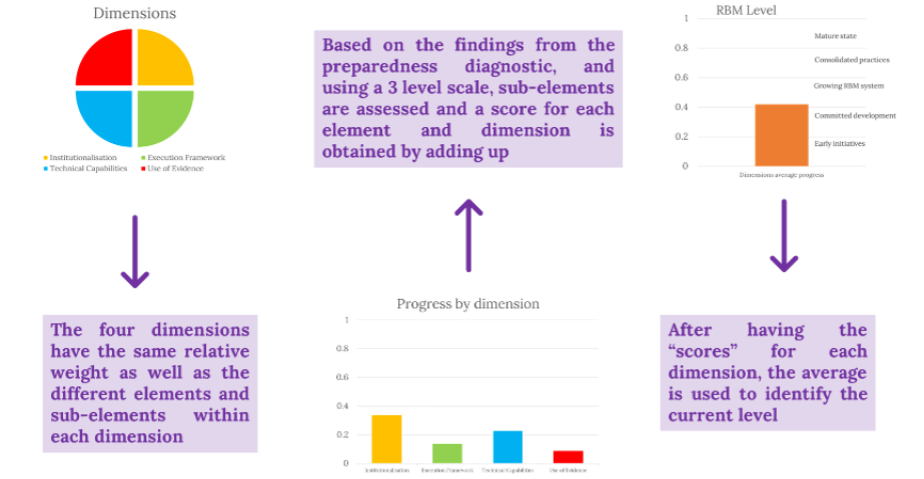
\includegraphics[width=1\linewidth]{./images/figure_8} 

}

\caption{How to identify the current level of the RBM system maturity}\label{fig:figure8}
\end{figure}

\begin{center}\rule{0.5\linewidth}{0.5pt}\end{center}

\hypertarget{appendixB}{%
\chapter{Detailed findings}\label{appendixB}}

In the following table, you can consult all the findings found in this PD in detail.

\begin{table}
\centering
\begin{tabular}[t]{l|l}
\hline
I. Institutionalisation Detailed Findings &  \\
\hline
\multicolumn{2}{l}{\textbf{1. There is a documented, approved and binding RBM Policy within the government:}}\\
\hline
\hspace{1em}1.1 It is relevant across the government at all levels & NA\\
\hline
\hspace{1em}1.2 It outlines guiding principles / pillars that are aligned to a results-oriented approach & NA\\
\hline
\hspace{1em}1.3 It communicates what RBM entails (e.g., clear definitions for key concepts) and clearly states how it works & NA\\
\hline
\hspace{1em}1.4 It identifies key actors who are responsible for the coordination and the measurement of the overall supervision and coordination of the RBM policy & NA\\
\hline
\hspace{1em}1.5 It identifies key actors who are responsible for supervising the implementation of the RBM policy and their functions (within MDAs) & NA\\
\hline
\hspace{1em}1.6 It is use-oriented in planning, budgeting, and implementing towards results, transparency and accountability & NA\\
\hline
\hspace{1em}1.7 The funding for M\&E activities and the responsible are identified & Although in the estimates of revenue \& expenditure 2020-2021 (which is the most recent one), there are specific estimates and funding towards M\&E. However, there is no identification of the M\&E activities to be undertaken nor the responsibles.\\
\hline
\multicolumn{2}{l}{\textbf{2. There are laws/regulations/norms* recognizing M\&E activities across the government}}\\
\hline
\hspace{1em}2.1 They are additional to the RBM Policy & NA\\
\hline
\hspace{1em}2.2 They delegate M\&E responsibilities to a single national body or to multiple MDAs & NA\\
\hline
\hspace{1em}2.3 It is relevant across the government at all levels and branches (e.g., scope of action) and defines the M\&E subjects & NA\\
\hline
\hspace{1em}2.4 They stablish that the M\&E results affect planning, budgeting and implementing activities & NA\\
\hline
\hspace{1em}2.5 (If more than one) They are consistent with each other & NA\\
\hline
\hspace{1em}2.6 It stablishes the need to designate focal points in each MDA across government & There are some monitoring activities within Saint Lucia´s government. However, there are no established or designated focal points in MDAs in charge of monitoring (and evaluation) activities.\\
\hline
\multicolumn{2}{l}{\textbf{3. There are guidelines that establish the rules and processes to perform monitoring activities:}}\\
\hline
\hspace{1em}3.1 They identify indicators types and the dimensions they want to measure (e.g. efficiency, efficacy), and monitoring tools (e.g. logic framework) to be developed for each project / social programme & The Medium Term Development Strategy 2020 - 2023 (MTDS) has a set of Key Performance Indicators, with yearly expected results, and presents a situation analysis for each of the six key results areas.\\
\hline
\hspace{1em}3.2 They identify specific timeframes to collect indicator data and develop monitoring tools to measure the indicators (e.g., collect every six months) for each project & The Medium Term Development Strategy 2020 - 2023 (MTDS) does not identify specific timeframes to collect indicator data and develop monitoring tools to measure the KPIs.\\
\hline
\hspace{1em}3.3 They have criteria to ensure data collection quality (design, measurement, report) & There are no criteria to ensure data collection quality.\\
\hline
\hspace{1em}3.4 They integrate the indicators as a monitoring system & There is no integration of the indicators to be tracked as a monitoring system.\\
\hline
\hspace{1em}3.5 The monitoring system has a stablished process to update its information periodically & NA\\
\hline
\hspace{1em}3.6 The monitoring system has a stablished process to update its indicators periodically & NA\\
\hline
\hspace{1em}3.7 There are rules providing all parts in the monitoring process with a way of presenting their opinion (e.g., institutional positions) & NA\\
\hline
\multicolumn{2}{l}{\textbf{4. There are guidelines that establish the rules and processes to perform evaluation activities:}}\\
\hline
\hspace{1em}4.1 They identify key stakeholders to be part of the evaluation process (e.g., evaluation process coordinators, evaluation subjects, evaluation process implementors) & There is no identification of key stakeholders to be part of the evaluation process.\\
\hline
\hspace{1em}4.2 They identify specific evaluation types & There is no identification of specific evaluation types according to necessities.\\
\hline
\hspace{1em}4.3 The identify specific timeframes for each evaluation type & NA\\
\hline
\hspace{1em}4.4 They identify specific characteristics and functions of evaluators & NA\\
\hline
\hspace{1em}4.5 It establishes an iterative process of evaluation (e.g., is not a one-time exercise) & There are no iterative processes of evaluation.\\
\hline
\hspace{1em}4.6 They identify the elements to be included in the evaluation's ToRs (e.g., objectives of the evaluation, the role and responsibilities of the evaluator and evaluation client and the resources available to conduct the evaluation) & There is no general knowledge of the elements to be requested/included in the evaluation ToRs.\\
\hline
\hspace{1em}4.7 They outline the operationalization process of the national evaluation agenda (e.g., it is agreed among relevant stakeholders) & There is no national evaluation agenda.\\
\hline
\hspace{1em}4.8 There have quality control mechanisms for evaluation activities (e.g., quality attribute listings, quality evaluations, peer review, satisfaction surveys, evaluate the evaluator) & There are no quality control mechanisms for evaluation activities.\\
\hline
\hspace{1em}4.9 There are rules providing all parts in the evaluation process with a way of presenting their opinion (e.g., institutional position) & NA\\
\hline
\multicolumn{2}{l}{\textbf{5. There are guidelines that establish the rules and processes to address and use of M\&E results}}\\
\hline
\hspace{1em}5.1 They identify instruments to measure the RBM System results & NA\\
\hline
\hspace{1em}5.2 They identify mechanisms to use monitoring results & NA\\
\hline
\hspace{1em}5.3 They identify mechanisms to use evaluation results & NA\\
\hline
\hspace{1em}5.4 They establish rules and processes that require the budgeting process to consider the results of M\&E activities (they make explicit the link between planning and budgeting) & There are no rules and processes that require the budgeting process to consider the results of M\&E activities.\\
\hline
\multicolumn{2}{l}{\textbf{6. There are formal actions towards building an enabling environment}}\\
\hline
\hspace{1em}6.1 There are key stakeholders identified as responsible for these formal actions & NA\\
\hline
\hspace{1em}6.2 There are strategies to enhance or attenuate positive or negative incentives for the use of monitoring & NA\\
\hline
\hspace{1em}6.3 There are strategies to enhance or attenuate positive or negative incentives for the use of evaluation & NA\\
\hline
\hspace{1em}6.4 There are mechanisms for the participation of stakeholders in the definition of monitoring activities and needs & NA\\
\hline
\hspace{1em}6.5 There are mechanisms for the participation of stakeholders in the definition of evaluation activities and needs & NA\\
\hline
\hspace{1em}6.6 There are periodic meetings involving relevant stakeholders to review the M\&E information as an RBM System feedback exercise & NA\\
\hline
\hspace{1em}6.7 There is a permanent strategy to communicate and sensitize about the benefits and challenges of M\&E & NA\\
\hline
\multicolumn{2}{l}{\textbf{7. There is a Results Oriented National Plan defined for a given period in the country:}}\\
\hline
\hspace{1em}7.1 It has defined objectives & The MTDS has defined objectives for each of the KRA.\\
\hline
\hspace{1em}7.2 It is constructed in a participatory process & The MTDS is constructed in a participatory process: public and private sectors take participation in its drafting.\\
\hline
\hspace{1em}7.3 It is constructed using the information generated by the RBM System & The MTDS is not constructed using the information generated by the RBM System.\\
\hline
\hspace{1em}7.4 It has defined strategies to implement the plan & The MTDS has not defined actions to implement the strategy itself.\\
\hline
\hspace{1em}7.5 It has defined indicators and monitoring tools by mandate, and they measure outcomes and outputs & The MTDS has defined KPIs for each KRA. Each KPI has annual targets and some initiatives related to them. Nevertheless, the tracking of the indicators is in terms of outputs, not outcomes.\\
\hline
\hspace{1em}7.6 It is evaluated by mandate & Although the MTDS has an M\&E framework that mentions the prioritization of monitoring and evaluation of priority projects, there is no mandate or standard that regulates M\&E activities.\\
\hline
\hspace{1em}7.7 It has specific evaluation activities & The MTDS has not specific evaluation activities.\\
\hline
7.8 It has defined responsible actors & The MTDS identifies the responsible actors for monitoring, mentioning their functions:

•   The Department of Economic Development, Transport and Civil Aviation is in charge of the Compliance Function with the following responsibilities:
• Advocacy for the adoption of project management standards for PSIP/priority projects  
• Revision of performance data and performance issues   
• Troubleshoot projects and make recommendations for corrective action  
• Liaise with implementing agencies to institute cor-rective actions    
• Provide project oversight 
• Ensure project alignment with national development strategies and strategic programs•         
• Document best practices from successful projects to include in the advocacy drive for project manage-ment standards and practices.    
• Compliance with donor requirement 
•   The Project Monitoring /Oversight committee is in chargeof the Accountability and Transparency function with the following responsibilities:
• Enforce the adaptation of project management poli-cies and standards for all projects 
• Liaise with PS committee and Cabinet for adoption of project management practices and procedures  
\hspace{1em}• Make recommendations to Cabinet to review or terminate projects for non-compliance with project standards\\
\hline
\hspace{1em}7.9 It considers regional (CARICOM) objectives & Even though there are no explicit links between the MTDS and CARICOM objectives, there is a connection between the regional actions undertaken and what the government of Saint Lucia plans for the development of the country.\\
\hline
\multicolumn{2}{l}{\textbf{8. There is a national budgeting strategy for a given period in the country:}}\\
\hline
\hspace{1em}8.1 It is allocated according to the objectives/goals/activities of the national planning & The national budget is allocated according to the objectives/goals/activities of the MTDS, considering the KRA and all the other government´s programmes.\\
\hline
\hspace{1em}8.2 It considers the prioritization of the objectives/goals/activities identified in the national planning & Even though the budget is allocated according to national objectives, its allocation is not improved using the information generated by evidence from the RBM System.\\
\hline
\hspace{1em}8.3 It is allocated using the information generated by evidence and the RBM System & Even though the budget is allocated according to national objectives, its allocation is not improved using the information generated by M\&E activities.\\
\hline
\hspace{1em}8.4 The budget allocation is defined in annual terms (e.g., it specifies the starting date, relevant milestones dates, and the end date) & The budget allocation is defined in annual terms.\\
\hline
\hspace{1em}8.5 It stablishes a specific allocation of resources for M\&E activities according to the budget period & The national budget does not have a specific allocation of resources for M\&E activities.\\
\hline
\hspace{1em}8.6 It considers other available information to define its allocation (e.g., national statistics/poverty measurements/etc.) & No, but the national budget considers the prioritization of the objectives/goals/activities identified in the MTDS, especially the ones related to the KRA.\\
\hline
\hspace{1em}8.7 The key actors and their responsibilities are clearly defined & The key actors and their responsibilities during the budgeting process are clearly defined. The Ministry of Finance, Economic Growth, Job Creation, External Affairs and the Public Service is the leader on this matter.\\
\hline
\end{tabular}
\end{table}

\begin{table}
\centering
\begin{tabular}[t]{l|l}
\hline
II. Execution Framework Detailed Findings &  \\
\hline
\multicolumn{2}{l}{\textbf{9. There are operative handbooks to implement the monitoring functions (i.e. Logic Framework):}}\\
\hline
\hspace{1em}9.1 They identify all the relevant activities to develop each stage of the process (e.g., Specific activities within the analysis of the project's context, stakeholder) & NA\\
\hline
\hspace{1em}9.2 They outline specific timeframes to implement every stage of the process & NA\\
\hline
\hspace{1em}9.3 They identify the responsible in every stage of the process (specific MDAs and units within the MDAs) & NA\\
\hline
\hspace{1em}9.4 They outline a dissemination strategy of the LF results (what, how, when and to who do you want to diffuse the results) & NA\\
\hline
\hspace{1em}9.5 The indicators are oriented to results and outcomes & The MTDS identifies six Key Results Areas (KRA): Agriculture, Citizen Security, Education, Healthcare, Infrastructure and Tourism. Each KRA has its indicators both at output and outcome levels.\\
\hline
\multicolumn{2}{l}{\textbf{10. There are operative handbooks that establish specific steps to develop each stage of the evaluation function:}}\\
\hline
\hspace{1em}10.1 They identify all the relevant activities to develop each stage of the evaluation process (e.g., evaluators selection, ToR definition for each evaluation, evaluation supervision) & NA\\
\hline
\hspace{1em}10.2 They outline specific timeframes to implement every stage of the process & NA\\
\hline
\hspace{1em}10.3 They outline a dissemination strategy of the evaluation results (what, how, when and to who do you want to diffuse the results) & NA\\
\hline
\hspace{1em}10.4 They identify the responsible (specific MDAs and units within the MDAs) in every stage of the process & NA\\
\hline
\multicolumn{2}{l}{\textbf{11. There is an operating and functioning coordination of M\&E at the national or/and subnational levels:}}\\
\hline
\hspace{1em}11.1 It is homogeneous across the government and holds a common language in concepts of M\&E & NA\\
\hline
\hspace{1em}11.2 It is integrated at various levels of government (national and subnational) & NA\\
\hline
\hspace{1em}11.3 It is known by all sectors and MDAs in government & NA\\
\hline
\hspace{1em}11.4 It is relevant (e.g., it recollects indicator data that is necessary, pertinent, and timely, it involves key stakeholders at different levels) & NA\\
\hline
\hspace{1em}11.5 It generates timely documents for specific evidence users & NA\\
\hline
\hspace{1em}11.6 It generates use-oriented documents for specific evidence users & NA\\
\hline
\hspace{1em}11.7 It is sufficiently funded (specific financial resources are allocated) & NA\\
\hline
\multicolumn{2}{l}{\textbf{12. There is a defined human resources structure for M\&E activities:}}\\
\hline
\hspace{1em}12.1 It has specific focal points in each MDA across the government & There are no specific M\&E focal points in each MDA. Nevertheless, each agency has an assigned chief economist, which get the monthly reports made by the agencies regarding performance.\\
\hline
\hspace{1em}12.2 The MDA focal points constitute a coordinated network that is part of the M\&E System & The MDAs focal points do not constitute a coordinated network.\\
\hline
\hspace{1em}12.3 The MDA focal points have clear functions, responsibilities and expected outcomes & These economists, which are the MDAs focal points, have not clear functions, responsibilities and expected outcomes.\\
\hline
\hspace{1em}12.4 The MDAs focal points become recognized strategic areas of information about the performance and impact of the MDAs projects / programmes & The MDAs focal points don't become recognized strategic areas of information about the performance and impact of the MDAs projects / programmes.\\
\hline
\end{tabular}
\end{table}

\begin{table}
\centering
\begin{tabular}[t]{l|l}
\hline
III. Technical Capabilities Detailed Findings &  \\
\hline
\multicolumn{2}{l}{\textbf{13. There are sufficient private and public entities providing M\&E services, including training, to the public sector.}}\\
\hline
\hspace{1em}13.1 They provide a variety of M\&E services (e.g., conduct diagnostics, evaluations, assessments) & The few entities in the region can provide M\&E and RBM services but do not in Saint Lucia.\\
\hline
\hspace{1em}13.2 MDAs demand those M\&E services based on their needs & There is practically no academic offer and demand for RBM capacity building.\\
\hline
\hspace{1em}13.3 They provide a broad academic offer for RBM capacity building (e.g., continuous courses / diplomas in M\&E topics, specific training to the public sector) & NA\\
\hline
\hspace{1em}13.4 There is an M\&E capacity building strategy demanding RBM training, which is periodic, targeted to the capacity building needs and with a whole-of-government approach & NA\\
\hline
\multicolumn{2}{l}{\textbf{14. There are skilled personnel in government with technical capacity and competencies to conduct planning and budgeting for results:}}\\
\hline
\hspace{1em}14.1 They have technical skills to use derived evidence from M\&E to improve planning (identify priorities, vulnerable population, what works to attend that priorities) & On average, the personnel have no technical skills to use derived evidence from M\&E (identify priorities, vulnerable population, what works to attend that priorities).\\
\hline
\hspace{1em}14.2 They have competencies to use M\&E results to define results-oriented budgeting (e.g., identify priorities, new public problems that should be addressed, policies that work, compare between policies) & The personnel do not have sufficient skills to use M\&E results to define results-oriented budgeting.\\
\hline
\hspace{1em}14.3 They have competencies to coordinate with other MDAs and relevant actors & The personnel have not that type of competencies. Also, it was mentioned that coordination and the "silo" culture between Ministries remains a key challenge to address when it comes to strengthening the RBM system.\\
\hline
\multicolumn{2}{l}{\textbf{15. There are skilled personnel in government with technical capacity and competencies to conduct monitoring activities:}}\\
\hline
\hspace{1em}15.1 They have technical skills to collect indicator data & There are no sufficient personnel with technical skills to collect indicator data.\\
\hline
\hspace{1em}15.2 They have technical skills to use monitoring tools & There are no sufficient personnel with technical skills to use monitoring tools.\\
\hline
\hspace{1em}15.3 They have the competences to identify monitoring needs in order to collect relevant, pertinent and timely data & The personnel have no sufficient competences to identify monitoring needs to collect relevant, pertinent and timely data.\\
\hline
\multicolumn{2}{l}{\textbf{16. There are skilled personnel in government with technical capacity and competencies to conduct evaluations and evaluation activities:}}\\
\hline
\hspace{1em}16.1 They have the competences to perform different evaluation types (e.g., design, process, impact) and use different methodologies (e.g., quantitative, qualitative, mixed methods) & On average, personnel have not the competences to perform different evaluation types (e.g. design, process, impact) and use different methodologies (i.e., quantitative, qualitative, mixed-methods).\\
\hline
\hspace{1em}16.2 They have the competences to identify evaluation needs and match them with proper evaluation types and methodologies: define evaluation horizon and ask relevant evaluation questions & The personnel have not the competences to identify evaluation needs and match them with proper evaluation types and methodologies: define evaluation horizon and ask relevant evaluation questions.\\
\hline
\hspace{1em}16.3 They have the competences to formulate reports that include relevant, pertinent, and timely information for different stakeholders & The personnel have not the competences to formulate reports that include relevant, pertinent and timely information for different stakeholders.\\
\hline
\hspace{1em}16.4 There is a capacity strengthening plan for on-going training in RBM and M\&E & There is not a capacity strengthening plan for on-going training in RBM and M\&E within the government.\\
\hline
\end{tabular}
\end{table}

\begin{table}
\centering
\begin{tabular}[t]{l|l}
\hline
IV. Use of Evidence Detailed Findings &  \\
\hline
\multicolumn{2}{l}{\textbf{17. RBM documents and goverment performance information are available and accesible for consultation}}\\
\hline
\hspace{1em}17.1 National planning documents and are publicly available & National planning documents and are publicly available, such as the MTDS.\\
\hline
\hspace{1em}17.2 National budget plans are publicly available & National budget plans and documents are publicly available, such as the Citizen´s Guide (to the 2021-2022 budget) and the Prime Minister´s Budget Address.\\
\hline
\hspace{1em}17.3 Documents that mention the results/findings/recommendations of monitoring and evaluation activities are publicly available & Documents that mention the results/findings/recommendations of monitoring and evaluation activities are not publicly available.\\
\hline
\hspace{1em}17.4 M\&E manuals / guidelines /ToRs are publicly available & M\&E manuals / guidelines /ToRs are not publicly available.\\
\hline
\hspace{1em}17.5 There is a dissemination strategy of evidence about government performance targeted to different stakeholders (e.g., citizens, parliamentarians, decision-makers, private sector, NGOs) & There is not a dissemination strategy of evidence about government performance.\\
\hline
\multicolumn{2}{l}{\textbf{18. There is an enabling environment for the use of M\&E results:}}\\
\hline
\hspace{1em}18.1 There are explicit positive or negative incentives for the use of monitoring results & NA\\
\hline
\hspace{1em}18.2 There are explicit positive or negative incentives for the use of evaluation results & NA\\
\hline
\hspace{1em}18.3 There are knowledge management practices & NA\\
\hline
\multicolumn{2}{l}{\textbf{19. M\&E results are systematically included in the planning \& budgeting:}}\\
\hline
\hspace{1em}19.1 They are used in an institutionalized way: they follow a established procedure & NA\\
\hline
\hspace{1em}19.2 There are action plans or other management instruments to ensure M\&E results/recommendations are implemented & NA\\
\hline
\hspace{1em}19.3 They justify the creation and design of government interventions & NA\\
\hline
\hspace{1em}19.4 They identify the target population of government interventions & NA\\
\hline
\hspace{1em}19.5 They identify general and specific recommendations to improve the implementation of government interventions & NA\\
\hline
\hspace{1em}19.6 They inform the design/redesign of government interventions & NA\\
\hline
\hspace{1em}19.7 They inform the initial budget allocations of government interventions & NA\\
\hline
\hspace{1em}19.8 They inform the budget increase/decrease/suspension of government interventions & NA\\
\hline
\hspace{1em}19.9 Evaluation findings/reports are updated periodically & NA\\
\hline
\hspace{1em}19.10 The M\&E results are used to define the MDAs budget & NA\\
\hline
\multicolumn{2}{l}{\textbf{20. The governemt has mechanisms to measure the use of the evidence that the RBM system generates}}\\
\hline
\hspace{1em}20.1 There are mechanisms to know how much the reports and publications on M\&E are downloaded or used by citizens & NA\\
\hline
\hspace{1em}20.2 There are use-of-evidence measurements to improve the use of M\&E results strategy & NA\\
\hline
\end{tabular}
\end{table}

\hypertarget{appendixC}{%
\chapter{Planning \& budgeting process}\label{appendixC}}

\hypertarget{national-budgeting-process-1}{%
\section[National budgeting process]{\texorpdfstring{National budgeting process\footnote{The Citizen's Guide to the 2021-2022 budget. Ministry of Finance, Economic Growth, Job Creation, External Affairs and the Public Service. Consulted in: \url{https://www.govt.lc/media.govt.lc/www/pressroom/news/attachments/the-citizen-s-guide-to-the-2021-2022-budget.pdf}}}{National budgeting process}}\label{national-budgeting-process-1}}

Saint Lucia's budgeting process consists of three main stages: 1. Budget planning and preparation; 2. Finalisation and 3. Budget implementation and monitoring. The stages are comprised as follow.

\hypertarget{budget-planning-and-preparation-1}{%
\subsection{Budget planning and preparation}\label{budget-planning-and-preparation-1}}

\begin{enumerate}
\def\labelenumi{\arabic{enumi}.}
\item
  The Ministry of Finance (MOF) prepares the Macroeconomic Outlook for the upcoming fiscal year where macroeconomic indicators are reviewed and projections for recurrent revenue, recurrent expenditure, and capital expenditure are formulated.
\item
  A request/call for new initiatives for recurrent revenue, recurrent expenditure as well as capital expenditure are sent to ministries.
\item
  The fiscal targets including economic indicators are established to determine revenue and expenditure projections, which aid in establishing overall spending limits for the new fiscal year.
\item
  The MOF issues the Estimates Call. In this circular, the preliminary allocations are outlined as well as other requirements of the MOF.
\item
  The Minister for Finance invites the private sector to submit inputs for the budget.
\item
  The agencies submit their new initiatives. The MOF reviews the submission and prepares recommendations in consultation with agencies.
\item
  Technical Budget Committee meetings are held with staff of the MOF and Department of Economic Development and Youth Economy to discuss recommendations, indicators and fiscal targets from the Budget Office, Debt Unit, Research Department and Department of Economic Development and Youth Economy. This committee then formulates recommendations and submits to the Budget Policy committee for approval through several iterations.
\end{enumerate}

\hypertarget{finalisation-1}{%
\subsection{Finalisation}\label{finalisation-1}}

\begin{enumerate}
\def\labelenumi{\arabic{enumi}.}
\setcounter{enumi}{7}
\item
  After extensive reviews and dialogue the MOF present the draft estimates to the Minister for Finance.
\item
  The Minister and Finance Officials meet with Cabinet to finalise the estimates.
\item
  A second call circular is sent to the agencies communicating cabinet final approval of the Budget and changes required to be reflected in the estimates book, and any other relevant instructions.
\item
  Following the Cabinet meeting, MOF prepares the printed estimates and develops the budget papers.
\item
  The Ministry for Finance prepares and submits a draft appropriation bill to the Attorney General
\item
  The Attorney General reviews the Appropriation Bill and prepares the Resolution.
\item
  Minister for Finance tables the Resolution in the House of Parliament.
\item
  Members of the Lower House debate the Estimates.
\item
  The Appropriation Bill is tabled and debated.
\item
  When passed the Appropriation Act is then assented to by the Governor-General and Gazetted.
\end{enumerate}

\hypertarget{budget-implementation-and-monitoring-1}{%
\subsection{Budget implementation and monitoring}\label{budget-implementation-and-monitoring-1}}

\begin{enumerate}
\def\labelenumi{\arabic{enumi}.}
\setcounter{enumi}{17}
\item
  The MOF sends out a call to agencies to submit their expenditure request (recurrent expenditure, capital), revenue (actual and projections), and procurement plans on a quarterly basis.
\item
  The MOF releases the allocation to agencies on a quarterly basis. The release of allocation is based in part on the current revenue performance and projections for the year. Capital expenditure allocation is determined based on the availability of the loan, grant, bond, or other fundraising and the status of the projects.
\item
  Agencies are required to submit monthly revenue reports and quarterly performance reports to the MOF.
\item
  The MOF is also required to produce and submit quarterly performance reports to the Minister for Finance.
\end{enumerate}

\hypertarget{appendixD}{%
\chapter{List of participants in the Preparedness Diagnostic}\label{appendixD}}

\begin{table}

\caption{\label{tab:unnamed-chunk-14}List of participants in the Preparedness Diagnostic}
\centering
\fontsize{15}{17}\selectfont
\begin{tabu} to \linewidth {>{\raggedright}X>{\raggedright}X>{\raggedright}X>{\raggedright}X}
\hline
Last name & First name & Organisation & Position\\
\hline
\textbf{Alcee} & Mandille & Performance Management \& Delivery Unit & Deputy Head\\
\hline
\textbf{Alcindor} & Pearl & Department of Economic Development & (Acting) Chief Economist\\
\hline
\textbf{Barnard} & Janet & Department of Economic Development, Transport and Civil Aviation & Deputy Permanent Secretary\\
\hline
\textbf{Bernard} & Karen & Attorney General's Chambers & Crown counsel\\
\hline
\textbf{Boshkovski} & Denis & The World Bank & Sr. Country Officer for the Eastern Caribbean countries\\
\hline
\textbf{Emmanuel} & Claudius & Department of Economic Development, Transport and Civil Aviation & Permanent Secretary\\
\hline
\textbf{Emmanuel} & Benjamin & Office of the Prime Minister & Cabinet Secretary\\
\hline
\textbf{Joseph Mathew} & Kerry & Department of Economic Development, Transport and Civil Aviation & Deputy Chief Economist\\
\hline
\textbf{Mathurin} & Cheryl & Department of Economic Development, Transport and Civil Aviation & Project Coordinator\\
\hline
\textbf{Rigobert} & Esther & Department of Finance & Permanent Secretary\\
\hline
\multicolumn{4}{l}{\rule{0pt}{1em}\textit{Note: }}\\
\multicolumn{4}{l}{\rule{0pt}{1em}Anonymously, +20 public servants answered the online questionnaires in various Saint Lucia´s MDAs. Their positions were: Permanent Secretaries, Deputy Permanent Secretaries, Directors, Managers, Budget and Planning accountable figure, and Project Managers.}\\
\end{tabu}
\end{table}

\hypertarget{appendixE}{%
\chapter{List of shared documents}\label{appendixE}}

Various and diverse documents were consulted on the official websites of the Government of Saint Lucia. Those that are for internal government use were shared through our Executive Coordinator and through information requests directly with the MDAs (via online questionnaires). These documents are:

\begin{itemize}
\item
  \textbf{Finance Administration Act (2005)}
\item
  \textbf{Listing of the House of Assembly and Cabinet of Ministers}
\item
  \textbf{Medium Term Development Strategy 2020-2023}
\item
  \textbf{Order of Precedence}
\item
  \textbf{Organisational chart of the Department of Commerce}
\item
  \textbf{Organisational chart of the Department of Finance}
\item
  \textbf{Organisational chart of the Department of Justice}
\item
  \textbf{Organisational structure of the Department of Agriculture}
\item
  \textbf{Public Procurement and Asset Disposal Act and Public Finance Management Act}
\item
  \textbf{Standard Operation Procedures (Department of Economic, Development, Transport \& Civil Aviation)}
\item
  \textbf{Strategic Plan 2020-2023 (Division of Economic Development)}
\end{itemize}

  \bibliography{book.bib,packages.bib}

\end{document}
